% Root-and-Branch working paper (RAB Kit, WS8). AI-generated research for Team Caplet - not a competition submission.
% Build: rab/paper/build.sh  (runs make_trace.py, then pdflatex + bibtex). Every number traces to rab/numbers*.yaml
% (keys shown as \nk{...}) or to a named results file (\src{...}); make_trace.py fails on any key or file it cannot find.
\documentclass[11pt,a4paper]{article}
\usepackage[T1]{fontenc}
\usepackage[utf8]{inputenc}
\usepackage{lmodern}
\usepackage{microtype}
\usepackage[a4paper,margin=2.3cm,headheight=14pt]{geometry}
\usepackage{graphicx}
\usepackage{booktabs}
\usepackage{tabularx}
\usepackage{longtable}
\usepackage{array}
\usepackage{xcolor}
\usepackage{enumitem}
\usepackage{fancyhdr}
\usepackage{caption}
\usepackage{placeins}
\usepackage{tikz}
\usetikzlibrary{positioning,arrows.meta}
\usepackage[round,authoryear]{natbib}
\usepackage[colorlinks=true,linkcolor=blue!50!black,citecolor=blue!50!black,urlcolor=blue!50!black]{hyperref}

\graphicspath{{../results/}}
\setlist{nosep,leftmargin=1.4em}
\captionsetup{font=small,labelfont=bf}
\setlength{\parskip}{0.35em}
\setlength{\parindent}{0pt}
\renewcommand{\arraystretch}{1.12}

% Trace macros: \nk = a key in rab/numbers*.yaml; \src = a results file (Gate-B reproduced). Checked by make_trace.py.
\makeatletter\g@addto@macro{\UrlBreaks}{\do\_\do\-\do\.}\makeatother
\newcommand{\nk}[1]{{\urlstyle{tt}\nolinkurl{#1}}}
\newcommand{\src}[1]{{\urlstyle{tt}\nolinkurl{#1}}}
\newcommand{\keys}[1]{\par{\footnotesize\raggedright\color{black!60}\textit{Traces to:} #1\par}}
\newcommand{\UNV}{\textsc{unverified}}

\newcommand{\banner}{AI-generated research for Team Caplet - not a competition submission}
\pagestyle{fancy}
\fancyhf{}
\fancyhead[C]{\footnotesize\textbf{\banner}}
\fancyfoot[C]{\footnotesize\thepage}
\renewcommand{\headrulewidth}{0.4pt}

\title{\vspace{-1.8em}\textbf{Root-and-Branch: evidence for a floor-plus-upside plan\\ for Laura Gao's commitments}\\[0.3em]
\large Working paper, RAB Kit}
\author{\normalsize RAB Kit (Claude Code, stream WS8) for Team Caplet\\ \normalsize Wharton Global High School Investment Competition 2026-27\\[0.2em]
\normalsize\fcolorbox{red!60!black}{red!4}{\parbox{0.86\textwidth}{\centering\textbf{\banner.}\\
The team writes every deliverable. Nothing here was executed in WInS, and the IPS was not edited.}}}
\date{\normalsize 30 September 2026 (Sydney). Market basis: U.S. Treasury par curve of 28 September 2026.}

\begin{document}
\maketitle
\thispagestyle{fancy}

\begin{abstract}
\noindent Laura Gao will invest \$300,000 in January 2027 and \$150,000 in January 2028. From that money she must
pay ten fixed \$50,000 operating payments (January 2033 to 2042) with a high degree of certainty, and she wants to
tell co-sponsors in 2031 a credible range for a 2033 facility gift. The team's adopted strategy, Root-and-Branch,
buys Treasuries dated to the ten payments with the first deposit (the root), buys a Treasury floor with part of the
second deposit, and puts the rest into one world stock fund (the branch). In 2031 co-sponsors hear a range from the
floor to the floor plus half the fund; the 2033 gift is capped at the top. This paper tests that plan; it does not
redesign it. On the 28 September 2026 curve the ten payments cost about \$289,000 (about \$292,000 on 1 January 2027),
the cheapest since mid-2002 and far below the roughly \$460,000 of 2020. Replaying 149 start years since 1872 and 13
stress scenarios on a zero-coupon basis, no payment is ever short, and once the floor is bought the gift never falls
below it. The 2031 top is typically about \$175,000; almost all of its uncertainty comes from Treasury yields at two
purchase dates, not from stocks. A pre-registered rule keeps the promised share at one half. The largest open issue is
that the securities Laura can actually buy pay coupons: they deliver the full \$500,000 only if coupons are
reinvested at about 5\%, so the plan must name who covers a shortfall. We list every decision the team must ratify
and classify each finding as \emph{fix before 6 Nov}, \emph{note in Final Report} or \emph{ignore}.
\end{abstract}

\vspace{-0.4em}
{\small\textbf{How to read the numbers.} Every figure is either a key in \texttt{rab/numbers*.yaml} (shown in grey
``Traces to'' lines, and listed with its value in Appendix~C) or a named, Gate-B-reproduced results file. ``MODEL''
means model output, not a market quote. Dollar figures are for \emph{Laura's plan} unless marked \emph{WInS book}.
Appendix~C is generated from the YAML files by \texttt{make\_trace.py}, which fails if any cited key or file is missing.}

% =====================================================================================================
\section{The client problem}

The case is short but strict. Laura invests \$300,000 at the
beginning of 2027 and \$150,000 at the beginning of 2028, and adds or withdraws nothing else before 2033. Four
requirements follow (Laura Gao 2026 Client Profile, pp.~2--4, in the team repository's \texttt{competition/official/2026\_27/}):

\begin{enumerate}
  \item \textbf{Ten operating payments} of a fixed \$50,000, one each January from 2033 to 2042, funded by the
  portfolio ``with a high degree of certainty'' and without outside funding. Teams must \emph{define} that
  certainty, say how they evaluated it, and name the assumptions behind it.
  \item \textbf{An operating reserve} set aside in January 2033: its size, what it holds, and how that changes.
  \item \textbf{A facility contribution} in 2033 that is responsible and leaves Laura financial flexibility.
  \item \textbf{A 2031 range} for that contribution, told to co-sponsors, with a stated confidence that the 2033 gift
  lands inside it, and which must not endanger the payments.
\end{enumerate}

The difficulty is the mix of horizons. The payments are fixed dollars due 6 to 15 years out: a pure liability. The
facility gift is a wish that should grow if markets are kind, but whose bottom must be credible two years before it
is paid. The competition portfolio (WInS: \$300,000 of virtual cash, \$25 per stock or ETF trade and \$10 per Treasury
trade, at most 200 trades, orders of at most twice a security's daily volume, U.S. Treasuries the only bonds, trading ends 6 November 2026; official competition guide and WInS rules) is an
\emph{implementation} of the strategy, not Laura's money; its gains are not added to her projections.

% =====================================================================================================
\section{The strategy: Root-and-Branch}\label{sec:strategy}

The adopted IPS names the plan Root-and-Branch: secure the roots (the payments and a facility floor) before
anything is invested in the branch (stocks). Figure~\ref{fig:plan} shows the money flow.

\begin{figure}[h]
\centering
\begin{tikzpicture}[font=\footnotesize, box/.style={draw, rounded corners=2pt, align=center, inner sep=4pt, minimum height=1.05cm},
  arr/.style={-{Stealth[length=2mm]}, thick}]
\node[box, fill=blue!8, text width=3.3cm] (d1) {\textbf{Jan 2027}\\ \$300,000 deposit};
\node[box, fill=blue!8, text width=3.3cm, below=0.9cm of d1] (d2) {\textbf{Jan 2028}\\ \$150,000 deposit\\ (+ any 2027 remainder)};
\node[box, fill=green!10, text width=5.0cm, right=1.0cm of d1] (root) {\textbf{Root}: ten Treasury holdings, each maturing\\ just before a \$50,000 payment\\ (bought latest payment first)};
\node[box, fill=green!10, text width=5.0cm, right=1.0cm of d2, yshift=0.35cm] (floor) {\textbf{Floor}: Treasuries repaying the\\ deposit by late 2032 (\$150,000)};
\node[box, fill=orange!15, text width=5.0cm, below=0.25cm of floor] (branch) {\textbf{Branch}: one world stock fund (VT),\\ held to 2033, never needed for a payment};
\node[box, fill=black!4, text width=3.6cm, right=0.9cm of floor, yshift=0.1cm] (y31) {\textbf{2031}: range told to\\ co-sponsors: floor to\\ floor + half the fund};
\node[box, fill=black!4, text width=3.6cm, below=0.3cm of y31] (y33) {\textbf{2033}: gift = floor + half\\ the fund, capped at the\\ announced top; Laura keeps\\ the other half};
\node[box, fill=black!4, text width=3.6cm, right=0.9cm of root] (pay) {\textbf{2033--2042}: the root\\ becomes the operating\\ reserve and pays out};
\draw[arr] (d1) -- (root);
\draw[arr] (d2.east) -- ++(0.45,0) |- (floor.west);
\draw[arr] (d2.east) -- ++(0.45,0) |- (branch.west);
\draw[arr, dashed] (d2.north) -- node[left, align=right, font=\scriptsize]{first completes the root\\ if yields fell before 2027} (d1.south);
\draw[arr] (root) -- (pay);
\draw[arr] (floor.east) -- (y31.west|-floor.east);
\draw[arr] (branch.east) -- (y33.west|-branch.east);
\end{tikzpicture}
\caption{Root-and-Branch as adopted. The strategy is fixed by the IPS; this paper tests it. The \emph{WInS book} is
the plan after both deposits scaled to \$300,000 (Sheet tab \texttt{Portfolio}): ten dated holdings (IBTM--IBTR and
five Treasury bonds dated 2037--2041), IBTM also carrying the floor, VT and a little cash.}
\label{fig:plan}
\end{figure}

\textbf{Why this shape.} It is the textbook answer to a problem with promised payouts: fund the promises with
safe assets held to maturity, and invest only the surplus in risky assets
\citep{leibowitz1986dedicated,dybvig1999protect}. Safety comes first in the sense of \citet{roy1952safety}: the
disaster outcome, a missed payment or a lost 2028 deposit, is made as unlikely as possible before any upside is
sought. The 2028 book is a buy-and-hold floor-plus-stocks position \citep{perold1988dynamic}: its worst case is set
by the floor, its upside by the market, and no trading rule is needed. In the language of constant proportion
portfolio insurance \citep{black1992cppi} it is CPPI with a multiplier of one and no rebalancing. Separating
must-pay money from could-grow money follows goals-based practice
\citep{shefrin2000bpt,chhabra2005beyond,das2010mental,das2018gbwm}, which treats the payments as ``needs'' and the
top of the range as a ``wish''.

\textbf{The WInS book.} The team's planned WInS book costs about \$294,800 at 28 September closes, including \$200 of
commission, leaving \$5,235.50 cash: dated Treasury holdings about 90\%, the world stock fund about 9\%, cash about 2\%
(\emph{WInS book}). Four independent pricers agree on this to the cent (Gate A, Appendix~B).
\keys{\nk{wins.portfolio.cost_close_0928}, \nk{wins.portfolio.split_close_0928}, \nk{wins.portfolio.holdings_close_0928}}

% =====================================================================================================
\section{Data}\label{sec:data}

All data are public, read-only and dated; hashes, URLs and fetch times are in \src{rab/data/MANIFEST.csv} and
\texttt{rab/data/history/MANIFEST.csv}. Table~\ref{tab:data} lists what each model uses.

\begin{table}[h]
\centering\small
\begin{tabularx}{\textwidth}{>{\raggedright}p{3.9cm}>{\raggedright}Xp{2.2cm}l}
\toprule
Data & Source (URL in manifest) & As of & Used by \\
\midrule
Daily Treasury par yield curve, 1990--2026 & U.S. Treasury, home.treasury.gov daily par yield curve CSV & 28 Sep 2026 & M1, M2, M5, M8, M9 \\
Constant-maturity yields 1962--1989; breakevens; CPI & FRED (fredgraph CSV) & 25 Sep 2026 & M2, M5, M7 \\
Long rate and CPI 1871--1961; monthly stocks & R.~Shiller, shillerdata.com (\texttt{ie\_data.xls}) & Sep 2026 & M3, M5, M7 \\
Annual U.S. returns 1928--2025 & A.~Damodaran, NYU Stern (\texttt{histretSP.xls}) & Jan 2026 & M3, M5, M6 \\
International returns 1871--2020 & Jord\`a--Schularick--Taylor Macrohistory Database R6 & R6 & M5, M6, M7 \\
Factor and regional returns & Kenneth French Data Library & Aug 2026 & M5, M6 \\
Capital market assumptions & J.P.~Morgan 2026 Long-Term Capital Market Assumptions (world stocks 7.0\% a year) & 30 Sep 2025 & M3, M6, M7 \\
iBonds facts (NAV, holdings, yield) & iShares product pages & 24--28 Sep 2026 & M1, M9 \\
ETF closes and volume & Nasdaq (primary), Yahoo Finance (secondary) & 28 Sep 2026 & M1, M9 \\
WInS prices and the book & Team Sheet tabs \texttt{Portfolio}, \texttt{Book L}, \texttt{WInS Notes} (read only) & 28--29 Sep 2026 & M1, M9 \\
\bottomrule
\end{tabularx}
\caption{Data. The reference curve has a 10-year yield of 5.24\% on 28 September 2026. WInS name strings for
IBTO--IBTR and the five bonds, the bond quantity unit and WInS accrued-interest conventions are \UNV{} until seen
in WInS; two WInS bond prices (4.5\% Feb-2036, 4.375\% Feb-2038) were stale on 29 September and are not traded.}
\label{tab:data}
\end{table}
\keys{\nk{market.par_curve}, \nk{wins.bond_check.*}, \nk{market.etf_2026-09-28}, \nk{ws3.inputs.mc}}

% =====================================================================================================
\section{Methods}\label{sec:methods}

Nine models answer nine questions (Table~\ref{tab:models}); each has a one-page card in Appendix~A. Three rules
governed all of them.
\begin{itemize}
  \item \textbf{Spec before code, rule before result.} Each model was specified in writing first. Where a model makes a
  decision (the promised share in M4, the fund switch in M6, the assumptions to state in M8), the decision rule was
  committed to git before any result existed.
  \item \textbf{Dual computation.} Every headline number was rebuilt blind from the spec by a second builder who never
  saw the first builder's code (Gate B), with tolerances fixed in advance (range ends $\pm$2\%, probabilities
  $\pm$2 points). The ladder was priced by four builders (Gate A).
  \item \textbf{One source of numbers.} Gate A locked \texttt{rab/numbers.yaml} with a hash; stream files add model
  outputs that passed Gate B. Seeds are fixed (20260930); \texttt{make -C rab all} rebuilds every number and figure.
\end{itemize}

\begin{table}[h]
\centering\small
\begin{tabularx}{\textwidth}{l>{\raggedright}p{4.3cm}>{\raggedright\arraybackslash}X}
\toprule
& Question & Method (card in Appendix A) \\
\midrule
M1 & What do the ten payments cost now? & Bootstrap zero curve from the official par curve (log-linear discount factors); price each payment and each WInS holding; yield-check WInS bond prices; coupon-reinvestment stress \\
M2 & Could the ladder cost over \$300,000 by January 2027? & Five estimators of 3-month rate moves: rescaled history, similar-yield history, Vasicek AR(1), three-factor PCA+VAR, options (MOVE) \\
M3 & What will the branch be worth, 2028--2033? & Monte Carlo, 200,000 paths each: fat tails (Student-$t$), Shiller block bootstrap, Bayesian uncertain mean (PyMC), lognormal reference \\
M4 & What share of the fund should be promised (D6)? & Pre-registered two-test rule on M3's paths; floor delivery model; NSGA-II front (pymoo) as a check \\
M5 & How would the plan have done in history? & Ladder priced on every curve since 1871; plan replayed from 149 start years (1872--2020) \\
M6 & Is a rival plan or another fund better? & Eight rivals and four fund alternatives on the same money and metrics; history + J.P.~Morgan Monte Carlo \\
M7 & What do bad episodes do? & 13 historical or hypothetical scenarios on today's curve; real value of the payments \\
M8 & Which assumptions move the range? & One-at-a-time tornado and Sobol indices (SALib) on the full chain \\
M9 & Which WInS security fills each slot? & Screen on maturity, price vs curve, coupon share, cost, 2$\times$-volume rule, name check \\
\bottomrule
\end{tabularx}
\caption{The nine models. M1 and M5--M7 are deterministic; M2--M4, M6 and M8 are Monte Carlo with seed 20260930.}
\label{tab:models}
\end{table}

\textbf{Two bases.} Laura's plan is modelled with zero-coupon Treasuries (STRIPS maturing 15 November before each
payment), which pay exactly \$50,000 and need no reinvestment. Under the team's reading of the rules (the FAQ heading
``Investments permitted (for BOTH contributions)'', reading R1(a) in \texttt{rab/assumptions.md}), Laura's real plan
may use only WInS-listed securities: iBonds ETFs and coupon Treasuries (``Book L''). Section~\ref{sec:coupons}
measures what that difference costs.

% =====================================================================================================
\section{Results}\label{sec:results}

\subsection{Ladder cost and the cost of certainty}\label{sec:ladder}

\textbf{Today.} On the 28 September 2026 curve the ten payments cost about \$289,000 in STRIPS (the headline basis),
or about \$292,000 carried forward to 1 January 2027. That leaves about \$7,600 of room under the \$300,000 deposit;
yields would have to fall about 26 basis points before January for the room to go. Valued on the payment dates
themselves (a liability value, not a price anyone can pay) the figures are about \$287,000 and \$290,000. Four
reasonable curve methods give \$292,000 give or take \$300 for the January figure, and an independent ChatGPT pricing
agreed within about \$200.
\keys{\nk{laura.ladder.cost_today_strips}, \nk{laura.ladder.cost_2027_strips}, \nk{laura.ladder.headroom_2027_strips},
\nk{laura.ladder.breakeven_fall_bp_strips}, \nk{laura.ladder.value_today_exact}, \nk{laura.ladder.value_2027_exact},
\nk{laura.ladder.cost_2027_strips_model_band}, \nk{laura.ladder.gpt_check}}

\textbf{The plan on today's curve.} Carried to January 2028, the root is about 66\% of Laura's money, the floor
about 25\% (about \$117,000 buys the \$150,000 floor at today's 5-year yield) and the stock fund about 9\%, about
\$41,000. The Sheet's typed split (65.9 / 24.3 / 8.7, plus 1 point of cash) is within 0.1 point of this.
\keys{\nk{laura.plan_split_2028.strips}, \nk{laura.floor_cost_2028}, \nk{laura.stock_fund_2028_usd.strips},
\nk{wins.portfolio.targets_typed}}

\begin{figure}[t]
\centering
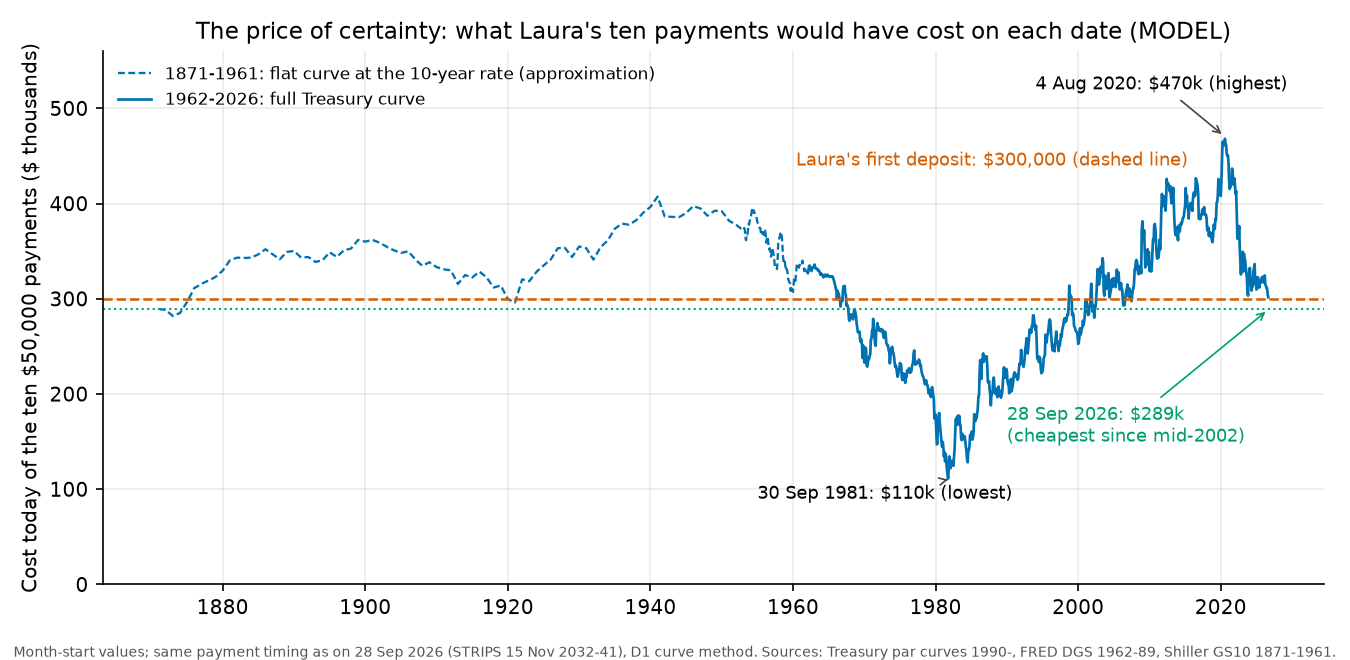
\includegraphics[width=0.92\textwidth]{M5/fig_cost_of_certainty.png}
\caption{The price of certainty (M5, MODEL). What the ten payments would have cost on each date with today's payment
timing. Before 1962 only a single long rate exists, so the curve is flat (dashed); on 1962--2026 this overstates the
cost by a median 0.8\%.}
\label{fig:coc}
\end{figure}

\textbf{History.} Figure~\ref{fig:coc} prices the same ten payments on every Treasury curve since 1871. On the daily
curves since 2000 (about 6,700 days), \$300,000 would have bought all ten payments on only about 1 day in 9; the
28 September price is the cheapest since mid-2002. At 2020 yields the ladder cost about \$460,000 (range \$408,000 to
\$470,000; the peak, about \$470,000 on 4 August 2020, is the dearest day since 1990). Even then the plan design
would have held: only on 197 of the 6,688 days, all in 2020--21, would part of one payment have been left unfunded
after both deposits, at worst about \$21,000. Over a longer window, only about one month in four since 1871
(23\%) was as cheap as today; the cheapest day was about \$110,000 on 30 September 1981.
\keys{\nk{history.days_priced_since_2000}, \nk{history.share_days_le_300k}, \nk{history.cheapest_since},
\nk{history.cost_2020_median}, \nk{history.cost_2020_range}, \nk{history.cost_max}, \nk{history.unfunded_days},
\src{rab/results/M5/M5_report.txt}}

\textbf{What this means.} Certainty is bought with Treasuries, so its price is set by the interest rate on the day
the money arrives. Today's rates are high by the standard of the last 150 years, which is why the first deposit can
buy all ten payments outright and still leave a \$150,000 floor and a stock fund.

\subsection{The ladder Laura can actually buy: coupons}\label{sec:coupons}

STRIPS have no coupons, so nothing needs reinvesting. The WInS-listed ladder (five iBonds ETFs and five coupon bonds)
receives part of its money early as coupons, which must be reinvested until each payment date. Table~\ref{tab:reinvest}
shows what the ten holdings deliver in total, as sized in the team's Sheet, at different reinvestment rates.

\begin{table}[h]
\centering\small
\begin{tabular}{lrr}
\toprule
Coupons reinvested at & Delivered by the ten holdings & Against \$500,000 \\
\midrule
Today's forward rates & about \$507,000 & over \\
Each holding's own yield (about 5\%) & about \$503,000 & over \\
Own yield minus 2 points & about \$479,000 & short \\
2\% & about \$466,000 & short \\
0\% & about \$447,000 & short \\
\bottomrule
\end{tabular}
\caption{Coupon reinvestment on Book L (M1 section E, MODEL). The ten total \$500,000 only if coupons earn about 5\%
or more. On the government's promise alone, each holding still delivers at least about \$42,000 of its \$50,000.
Keeping every payment whole if coupons earn only 2\% would cost about \$20,000 more of the same holdings today, more
than the \$7,600 of room.}
\label{tab:reinvest}
\end{table}
\keys{\nk{reinvest.bookL_delivered}, \nk{reinvest.rung.*}, \nk{reinvest.bookL_buffer_cost},
\nk{ws3.external.ws7_coupon_reinvestment}}

Two points soften this. First, sized to pay exactly \$50,000 a year at forward rates, the WInS-listed ladder costs
about \$289,200, within \$100 of STRIPS, so it is not more expensive; the risk is in the reinvestment, not the price.
Second, lower-coupon bonds (1.375\% Nov-2040, 2.000\% Nov-2041), if WInS lists them, cut the share of cash arriving as
coupons from 38\% to 17\% and from 33\% to 24\% on those two rungs (M9). The honest definition of ``a high degree of
certainty'' therefore has two parts: the U.S. government owes most of each payment, and a named part of the portfolio
covers any reinvestment shortfall before the facility gift (Section~\ref{sec:decisions}).
\keys{\nk{ws4.bookL_cost_resized}, \src{rab/trades/M9_selection.md}}

\subsection{The 2031 range and the promised share (D6)}\label{sec:range}

\textbf{Where the range sits.} The bottom of the range is an owned bond; the top is the floor plus half the stock
fund on the day. Figure~\ref{fig:range} shows the top under four return models. The typical top is about \$175,000;
in 90\% of paths it lies between about \$165,000 and \$190,000. The choice of stock model moves the typical top by
less than \$1,000, because only about 9\% of Laura's money is in stocks and only half of that is promised.
\keys{\nk{ws2.range.top2031}, \nk{laura.plan_split_2028.strips}}

\begin{figure}[t]
\centering
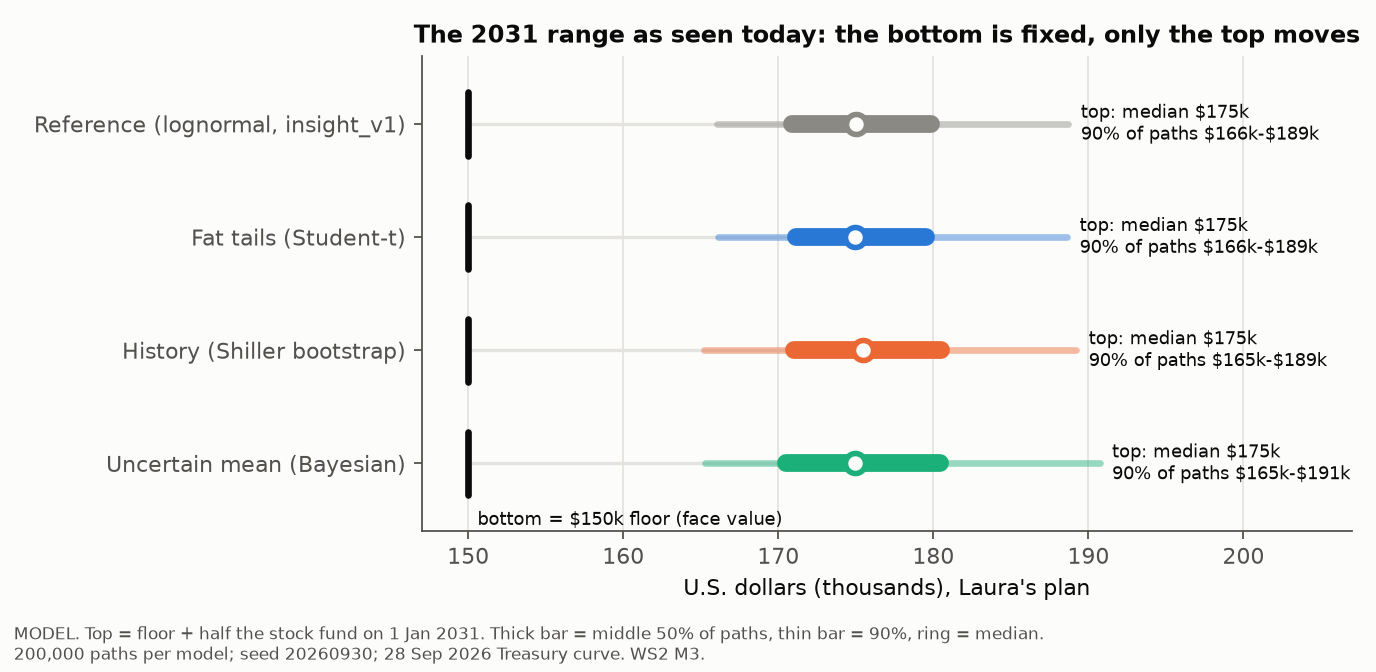
\includegraphics[width=0.84\textwidth]{M3/fig_M3_top2031.png}
\caption{The 2031 range as seen today (M3, MODEL; 200,000 paths per model). The bottom is the floor; only the top
moves. The figure draws the floor at its \$150,000 face value; the range memo quotes it as \$145,000 (see text).}
\label{fig:range}
\end{figure}

\textbf{Will the gift land inside the range?} By construction, yes, if five things hold: (1) the floor holding pays at
least the quoted bottom; (2) the 2028 deposit arrives; (3) the gift is capped at the top; (4) no cost is taken from
the floor; (5) any coupon shortfall is covered before it reaches the floor. No gift fell outside its range in 1.6
million model paths. The models only add \emph{where} it lands: about 3 times in 4 at the top or within about \$3,700 of
it, about \$2,000 below the top on average, and below the middle at most about 1 time in 200. In about 1 case in 5
the fund is worth less in 2031 than it cost in 2028; the range is then narrower, but its bottom does not move.
\keys{\nk{ws2.range.gift_inside_range}, \nk{ws2.range.p_fund_holds_2031_to_2033}, \nk{ws2.range.expected_short_of_top},
\nk{ws2.range.p_below_middle}, \nk{ws2.range.p_fund_below_cost_2031}}

\textbf{Quote the floor rounded down.} An iBonds fund is not a zero-coupon bond: modelled with realistic
reinvestment and its 0.07\% fee, the floor holding pays about \$149,000 in a typical case and at least about \$146,000,
and falls short of \$150,000 about 2 times in 3. Quoting the bottom as \$145,000 (the worst case rounded down to
\$5,000) keeps ``the gift cannot fall below the bottom'' literally true.
\keys{\nk{ws2.range.floor_delivery}, \nk{ws2.range.announced_floor}, \nk{ws2.range.floor_shortfall_vs_face}}

\textbf{How much to promise.} The pre-registered rule (committed before any M4 result) takes the largest share
of the fund that passes two tests in all three decision models: the gift stays above the announced \$145,000 in
99.5\% of paths, and Laura keeps at least 10\% of her gift in 95\% of paths. The answer is 0.50, 0.47 and 0.47, so
0.47; the rule keeps ``half'' when the answer lies in 0.40--0.60 (Table~\ref{tab:d6}, Figure~\ref{fig:sprofile}). Raising the share never makes a broken
promise more likely: no path puts the gift below \$145,000 at any share. It only moves dollars from Laura's cushion
to the gift, one for one. The answer depends on Laura's taste for flexibility, not on the stock model: a 5\%
cushion would allow about 0.72, a 15\% cushion about 0.23.
\keys{\nk{ws2.d6.s_star}, \nk{ws2.d6.decision_share}, \nk{ws2.d6.p_gift_below_145k_any_share}, \nk{ws2.d6.options},
\nk{ws2.d6.rule_sensitivity}, \nk{ws2.d6.half_vs_047_expected_gift}}

\begin{table}[h]
\centering\small
\begin{tabularx}{\textwidth}{>{\raggedright}X>{\centering}p{2.6cm}>{\centering}p{3.3cm}>{\centering\arraybackslash}p{3.3cm}}
\toprule
Share of the fund promised & Expected gift & Laura keeps $\ge$10\% of her gift & She keeps, 1-in-20 bad case \\
\midrule
1/3 & about \$166k & 98--99\% of paths & about \$21k--\$22k \\
0.47 (the rule's answer) & about \$173k & 95--97\% & about \$16k--\$18k \\
\textbf{1/2 (adopted)} & \textbf{about \$174k} & \textbf{93--95\%} & \textbf{about \$15k--\$17k} \\
2/3 & about \$183k & 69--71\% & about \$10k--\$11k \\
All & about \$199k & 17--21\% & \$0 \\
\bottomrule
\end{tabularx}
\caption{D6 options (M4, MODEL; ranges span the fat-tail, history and uncertain-mean models). Two builds and ten
extra seeds give the same answer.}
\label{tab:d6}
\end{table}

\begin{figure}[h]
\centering
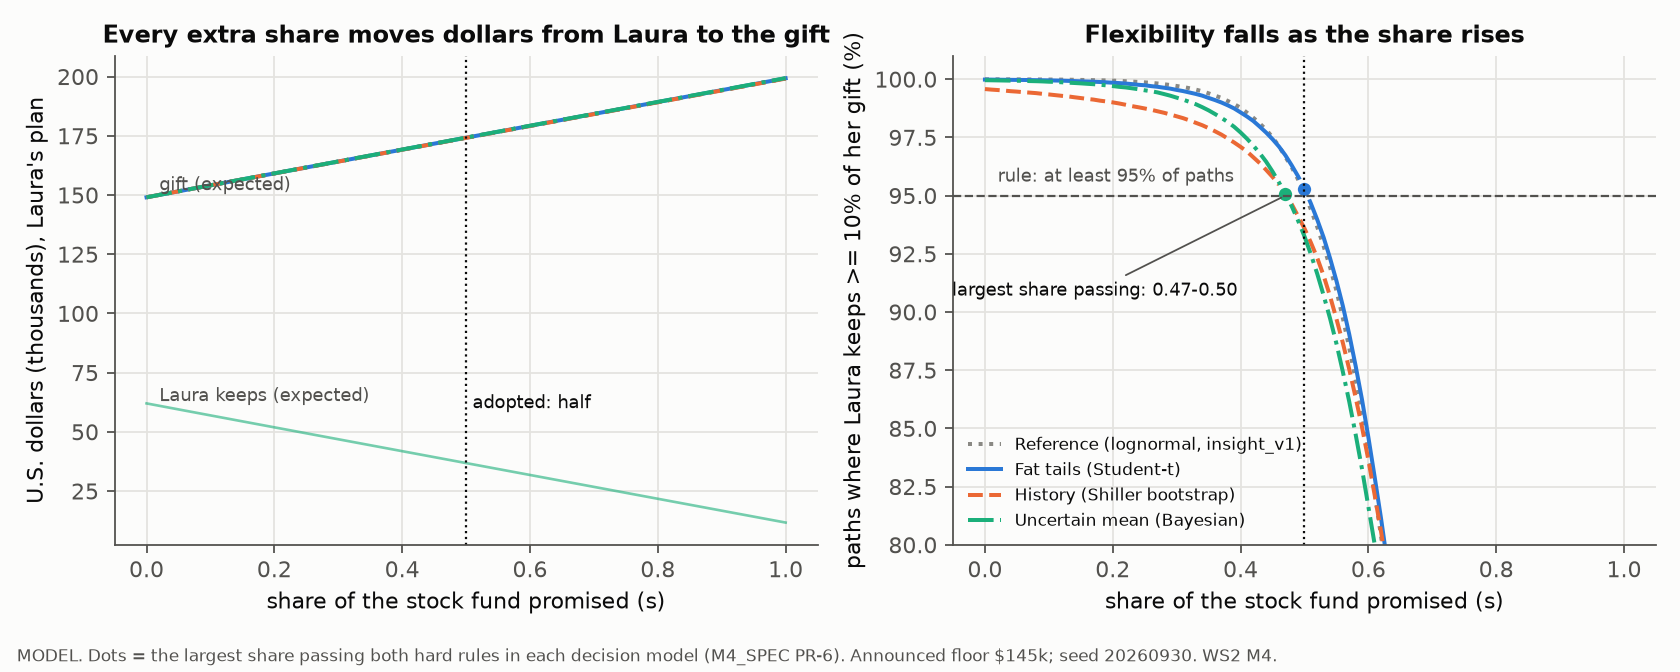
\includegraphics[width=0.9\textwidth]{M4/fig_M4_s_profile.png}
\caption{The promised share (M4, MODEL). Left: each extra share moves expected dollars from Laura to the gift.
Right: the share of paths in which Laura keeps at least a tenth of her gift; the pre-registered bar is 95\%.}
\label{fig:sprofile}
\end{figure}

\textbf{Coupons and the share.} With Book L instead of STRIPS, someone must pay a coupon shortfall. The kit's working
rule (Laura's kept half first, then the gift above the floor, then the floor) keeps half at today's yields (largest
passing share 0.42) and never lowers the 2031 top. If coupons earn 2 points less for years, no share passes, not even
zero, the top is lowered in 7--10\% of paths and the gift falls below \$145,000 in at most about 1 path in 300; at
2\%, the top is lowered in about 7 paths in 10. The share is not the lever for this risk; the holdings are.
\keys{\nk{ws2.d6.gap_owner}, \nk{ws2.d6.gap_owner_tolerance}, \nk{ws2.d6.ladder_gap}}

\subsection{Rivals and fund choice}\label{sec:rivals}

Every rival got the same money, the same ten payments and the same 2031 rule (M6). The case sets two hard tests:
the payments with a high degree of certainty, and a 2031 range that protects them. Table~\ref{tab:rivals} and
Figure~\ref{fig:rivals} show that only Root-and-Branch and an all-Treasury plan pass both.

\begin{table}[h]
\centering\small
\begin{tabularx}{\textwidth}{>{\raggedright}p{3.6cm}>{\raggedright}X>{\raggedright}p{2.1cm}cc}
\toprule
Plan & A payment short (Monte Carlo / 149 start years) & Certain in 2031 & 2033 money, \$k (5th/50th/95th) & Trades \\
\midrule
\textbf{Root-and-Branch} & never / 0 & \$150k & 181 / 207 / 252 & 13 \\
All-Treasury & never / 0 & about \$202k & 191 / 202 / 213 & 12 \\
Ladder + 60/40 & never / 0 & nothing & 154 / 216 / 307 & 21 \\
CPPI, multiplier 3 & never / 0; misses the \$150k in 2.0\% & nothing & 153 / 199 / 408 & up to 72 \\
60/40, whole portfolio & 1.3\% / 2 & nothing & 53 / 245 / 527 & 24 \\
Glide path 65$\to$20 & 0.17\% / 3 & nothing & 88 / 233 / 434 & 24 \\
Growth-first 75$\to$40 & 2.2\% / 3 & nothing & 36 / 249 / 571 & 24 \\
TIPS ladder & 60\% of inflation paths / 92 of 140 & \$150k & as adopted & 13 \\
\bottomrule
\end{tabularx}
\caption{Rivals on the same metrics (M6, MODEL, zero-coupon basis for every plan's payments). ``2033 money'' is what
is left for the facility and Laura once the payments are secured; Monte Carlo on J.P.~Morgan 2026 assumptions,
200,000 paths.}
\label{tab:rivals}
\end{table}
\keys{\nk{ws3.rivals.REC}, \nk{ws3.rivals.R1}, \nk{ws3.rivals.R2}, \nk{ws3.rivals.R3}, \nk{ws3.rivals.R4},
\nk{ws3.rivals.R4b}, \nk{ws3.rivals.R5}, \nk{ws3.rivals.R6_tips}}

\begin{figure}[t]
\centering
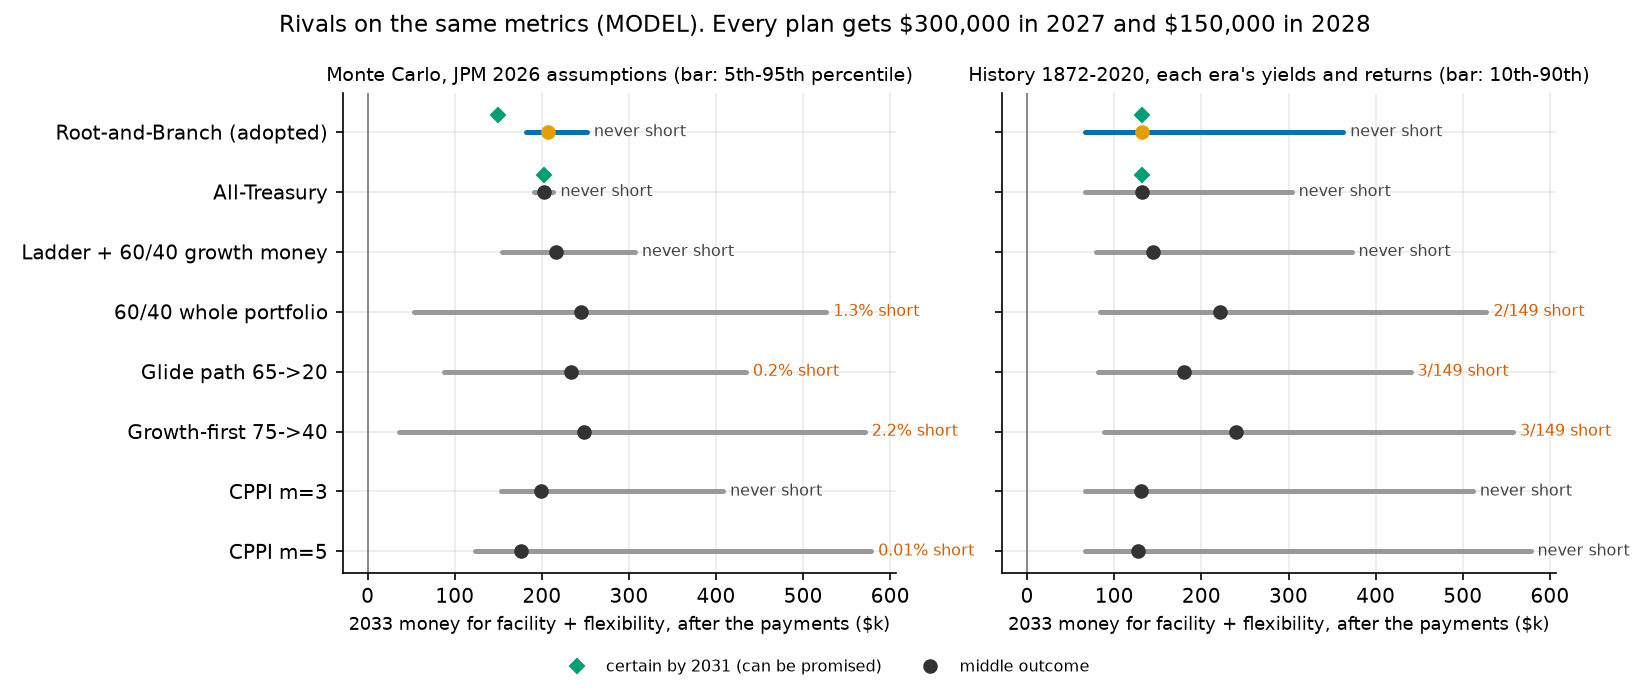
\includegraphics[width=\textwidth]{M6/fig_m6_rivals.png}
\caption{Rivals (M6, MODEL). Diamonds mark what can be promised with certainty in 2031.}
\label{fig:rivals}
\end{figure}

Plans without dated holdings earn more in the middle but leave a payment short in some paths and can promise nothing
in 2031. CPPI buys after rises and sells after falls: a fatter good case, a lower middle, and a floor that can break.
A TIPS ladder protects purchasing power Laura did not promise and puts at risk the dollars she did; it would need to
be about 1.43 times as large (about \$125,000 more) to pay every payment in 95\% of inflation paths.

\textbf{The closest rival, stated honestly.} All-Treasury has about the same typical 2033 money (about \$202,000
against \$207,000), a better bad case (about \$9,500 more at the 5th percentile) and a larger certain sum; for the
facility alone it gives more at every percentile, about \$28,000 more at the median, because it promises all its money.
Root-and-Branch trades that for about \$38,000 more in a good case, and for leaving Laura half the fund (about \$32,000
in the base case) as flexibility, which the case asks for. It is the only plan tested that passes both hard tests and
still holds stocks with money no payment relies on. The finding supports the IPS and needs no change.
\keys{\nk{ws3.rivals.rec_minus_all_treasury_mc}, \nk{ws3.rivals.facility_gift_rec_vs_all_treasury_mc},
\nk{ws3.rivals.stress_rec_vs_all_treasury}, \nk{ws3.stress.S0}}

\textbf{Which stock fund.} Four alternatives to VT were tested against a switch rule written first: switch only if
the bad-case gift rises by \$2,000 or more, or its spread narrows by 10\% or more, on every seed, with history
agreeing. None qualifies (Table~\ref{tab:fund}). Gold and REITs came closest (spread ratio 0.899 against a 0.90 bar,
passing on about 4 seeds in 5), partly by trimming the good case, and added nothing on real ETF prices 2012--2025. The
fund is small on purpose, so the choice barely matters: \textbf{keep VT}, ``one fund that owns the world's stock
market, left alone until 2033'' \citep{sharpe1991arithmetic,doeswijk2014global}.

\begin{table}[h]
\centering\small
\begin{tabularx}{\textwidth}{>{\raggedright}X>{\centering}p{3.4cm}>{\centering}p{3.0cm}>{\raggedright\arraybackslash}p{3.0cm}}
\toprule
Alternative to VT & Bad-case gift change (MC / history) & Spread vs VT (MC / history) & Rule \\
\midrule
VTI + VXUS (62/38) & +\$279 / +\$190 & 0.98 / 0.98 & keep VT \\
U.S. only & $-$\$61 / $-$\$1,481 & 0.98 / 1.02 & keep VT \\
Small/value tilt & $-$\$78 / +\$812 & 1.02 / 1.10 & keep VT \\
VT + 10\% gold + 10\% REITs & +\$1,164 / +\$1,388 & 0.899 / 0.80 & keep VT (not seed-robust) \\
\bottomrule
\end{tabularx}
\caption{Fund choice (M6, MODEL). VT's own bad-case gift is about \$165,000 and its typical gift about \$174,000.}
\label{tab:fund}
\end{table}
\keys{\nk{ws3.fund.alt.A1}, \nk{ws3.fund.alt.A2}, \nk{ws3.fund.alt.A3}, \nk{ws3.fund.alt.A4}, \nk{ws3.fund.vt_gift_mc},
\nk{ws3.fund.gold_reit_noise_free}, \nk{ws3.fund.gold_reit_etf_lens}, \nk{ws3.fund.max_abs_badcase_change}}

\subsection{Stress}\label{sec:stress}

M7 moves today's curve the way yields moved in past episodes, runs that episode's stock returns through the fund, and
follows the adopted rules (Figure~\ref{fig:stress}). On the zero-coupon basis, \textbf{every payment is paid in every
scenario}: once bought and held to maturity, a Treasury pays in full whatever its price does in between. Replaying
history's returns with today's yields from all 149 start years gives the same answer; the worst stretch (a fund bought
in 1929) still gives a gift of about \$159,000, the typical one about \$176,000, and the top is reached in 85\% of years.
\keys{\nk{ws3.stress.today_yields_backtest}, \nk{ws3.stress.worst_gift_once_floor_bought}}

\begin{figure}[t]
\centering
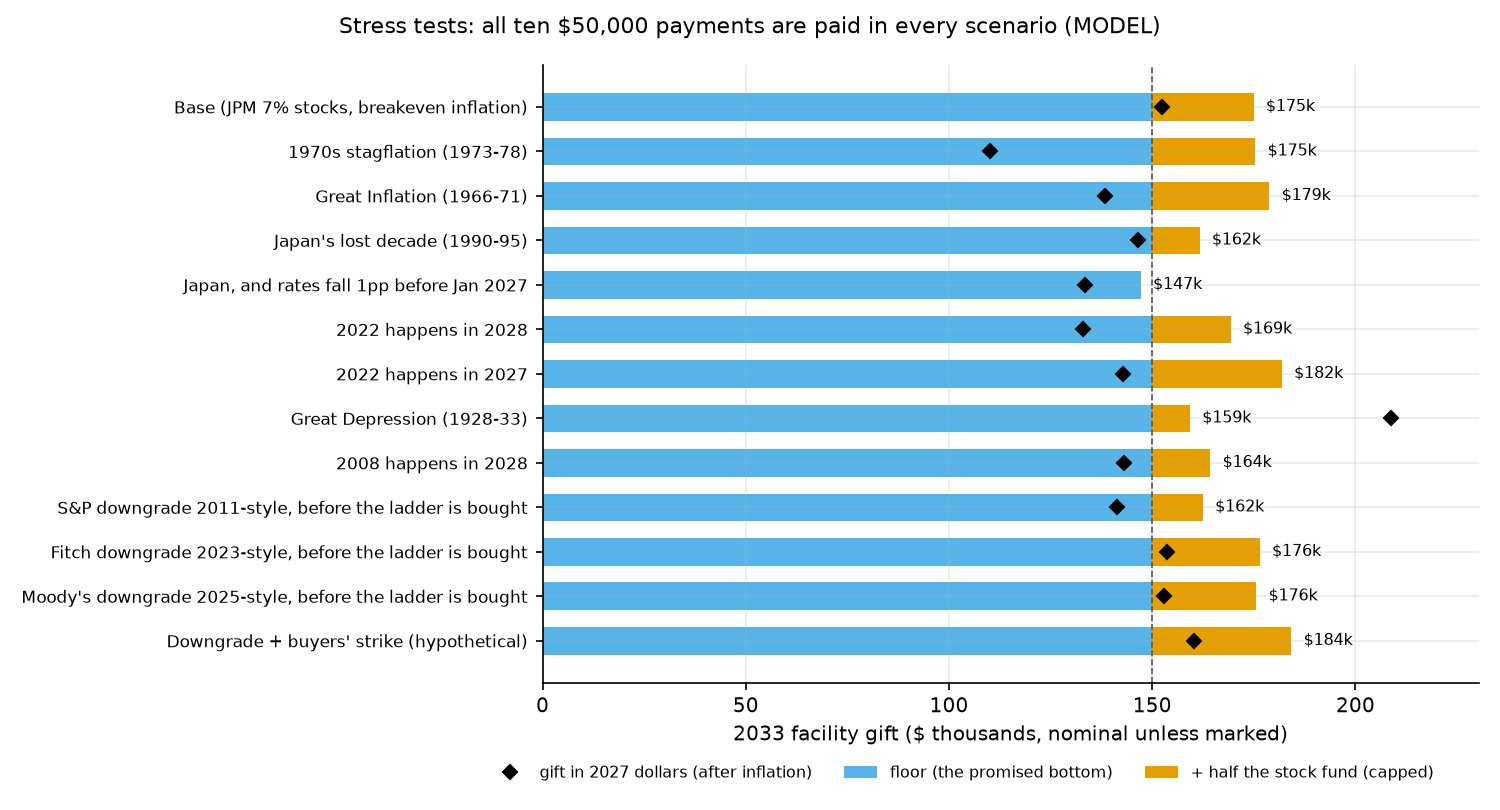
\includegraphics[width=0.93\textwidth]{M7/fig_m7_stress.png}
\caption{Stress tests (M7, MODEL). Blue: the floor; orange: half the stock fund, capped. Diamonds: the gift in 2027
dollars.}
\label{fig:stress}
\end{figure}

\textbf{The danger is before the money arrives.} A parallel fall in yields before January 2027 that lasts into 2028
needs a top-up from the 2028 deposit beyond about 26bp, uses up the stock fund at about 109bp (the floor still
\$150,000 under the kit's fixed-floor reading), and leaves a payment unfunded only beyond about 428bp. The worst replay
is Japan's lost decade with a 1-point fall first: the floor becomes about \$147,000 and there is no fund. A 2011-style
flight to safety (the 10-year yield fell about 56bp after the S\&P downgrade) would push the ladder to about \$309,000
and cost about \$20,000 of stock fund, but no payment.
\keys{\nk{ws3.stress.thresholds_bp}, \nk{ws3.stress.S2b}, \nk{ws3.stress.S4a}, \nk{ws3.stress.downgrades_dy10_bp},
\nk{ws3.stress.worst_gift_13_scenarios}}

\textbf{Stocks and coupons can fall together.} Table~\ref{tab:stresscoupon} pairs M7's episodes with the coupon gap
from Section~\ref{sec:coupons}: if coupons earn only 2\% for years, the gap (about \$30,000 in 2033 money) exceeds
Laura's kept half after a 2008, 1929 or Japan-style fall. At today's yields the gap (about \$1,600) never does.

\begin{table}[h]
\centering\small
\begin{tabularx}{\textwidth}{>{\raggedright}X>{\centering}p{2.4cm}>{\centering}p{2.0cm}>{\centering}p{2.0cm}>{\centering\arraybackslash}p{3.0cm}}
\toprule
Episode replayed from 2028 & 2031 range & 2033 gift & Laura keeps & Coupons at 2\%: gap beyond her half \\
\midrule
Base (J.P.~Morgan 7\% stocks) & \$150k--\$175k & about \$175k & about \$32k & none \\
2008 happens in 2028 & \$150k--\$164k & about \$164k & about \$18k & about \$12k \\
Japan 1990--95 & \$150k--\$163k & about \$162k & about \$12k & about \$19k \\
Great Depression 1928--33 & \$150k--\$159k & about \$159k & about \$17k & about \$13k \\
\bottomrule
\end{tabularx}
\caption{Stress with coupons (M7 + M1 E, MODEL; pairing by hand, one build).}
\label{tab:stresscoupon}
\end{table}
\keys{\nk{ws3.stress.S0}, \nk{ws3.stress.S6}, \nk{ws3.stress.S2}, \nk{ws3.stress.S5}, \nk{ws3.stress.coupon_gap_vs_laura_half}}

\textbf{Inflation stays with Laura.} The payments are fixed in dollars, as the case specifies. At the market's
expected inflation (2.34\%) the 2042 payment buys what about \$35,000 buys in 2027; in a 1970s-style decade, about
\$18,000 \citep[the qualification in][]{campbell2001longterm}. The IPS already says inflation erodes the floor's real
value; the Final Report should show these figures.
\keys{\nk{ws3.stress.real_value_payments}}

\subsection{Timing risk before January 2027}\label{sec:timing}

The first deposit arrives in January 2027; if yields fall first, the ten holdings cost more. Five estimators of
three-month rate moves, none taking a view on direction, put the chance that the ladder costs more than \$300,000 on
1 January 2027 at \textbf{about 1 in 3} (27--33\%; Figure~\ref{fig:timing}). If there is a shortfall it is typically
about \$10,000, about \$18,000 or more in 1 path in 20, and a whole payment waits in under 0.3\% of paths. The
earlier ``1 in 3'' from insight\_v1 survives, but for new reasons: higher yields on 28 September widened the room,
while today's rate volatility (MOVE index about 102) is higher than 2026's calm average.
\keys{\nk{ws4.gap_odds_2027}, \nk{ws4.gap_odds_2027_range}, \nk{ws4.gap_if_any_typical}, \nk{ws4.gap_p95},
\nk{ws4.p_whole_payment_waits}, \nk{ws4.move_index}, \src{rab/results/M2/m2_estimators.csv}}

\begin{figure}[h]
\centering
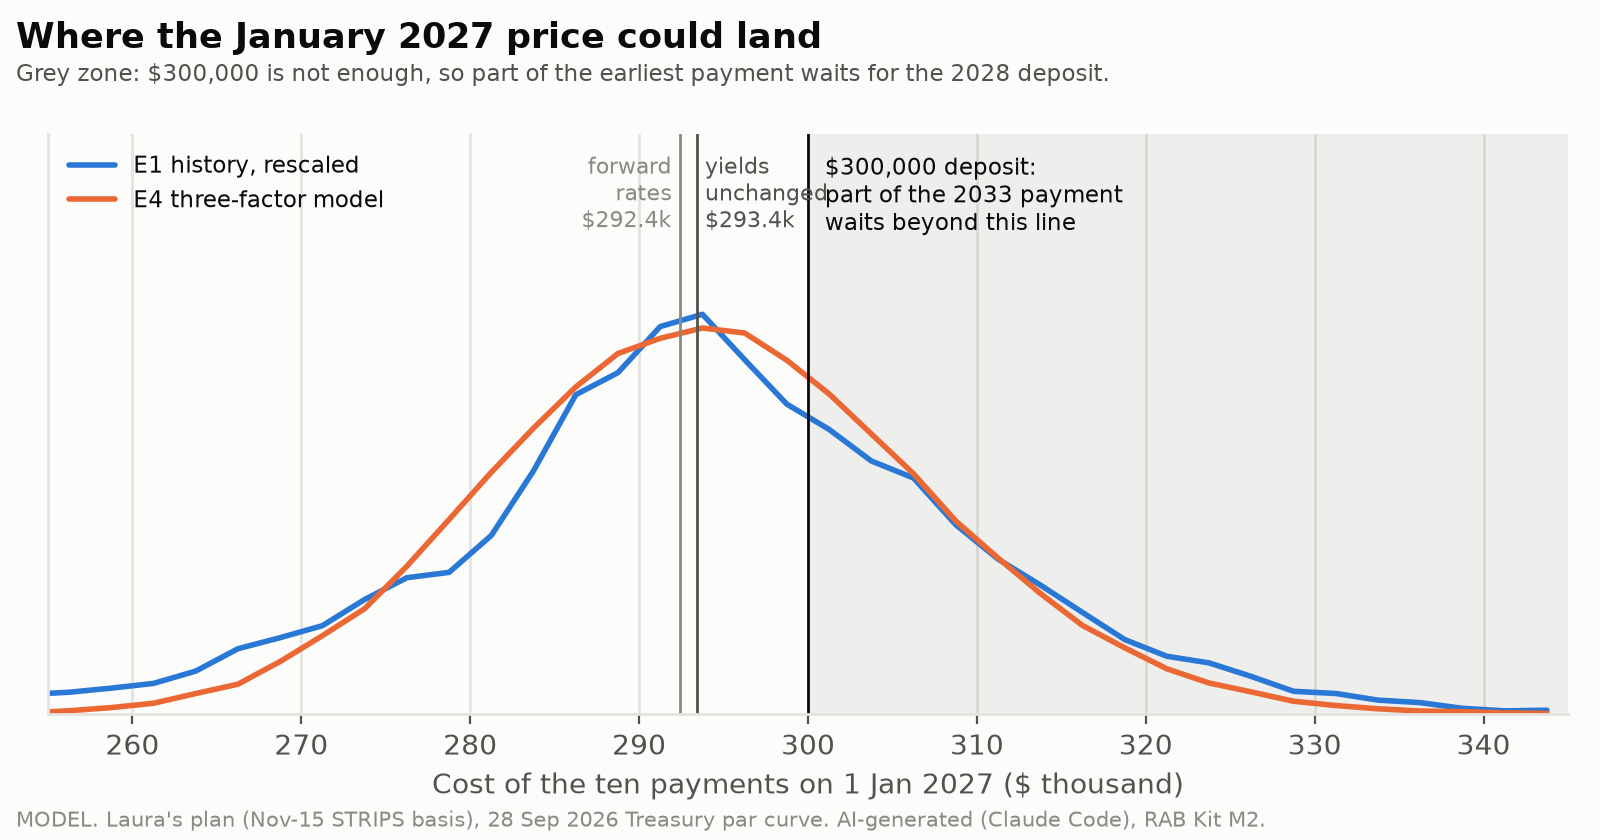
\includegraphics[width=0.78\textwidth]{M2/m2_fig3_cost_distribution.png}
\caption{Where the January 2027 price could land (M2, MODEL, STRIPS basis). Beyond \$300,000, part of the 2033 payment
waits for the 2028 deposit.}
\label{fig:timing}
\end{figure}

\textbf{Should Laura hedge?} No. Every hedging tool (futures, forwards, swaps, options, borrowing) is outside the
rules under the team's reading, and the design already absorbs the risk: buy all ten holdings at once, latest payment
first; any gap is the first call on the 2028 deposit and lands on the stock fund, which is typically about \$41,000 on
1 January 2028 and under \$20,000 in about 1 path in 6. A perfect hedge would gain at most about \$1,000 in expectation
and give away the fund's upside if rates rise. The rate move is settled by January 2028, three years before the range
is announced: it sizes the range but cannot break a promise.
\keys{\nk{ws4.stock_fund_2028_median}, \nk{ws4.p_stock_fund_below_20k_2028}, \nk{ws4.perfect_hedge_expected_gain},
\nk{ws4.topup_2028_after_150bp_fall}}

\subsection{Sensitivity: what moves the range}\label{sec:sensitivity}

M8 rebuilds the whole chain from the January 2027 purchase to the 2031 range and moves one assumption at a time
(Figure~\ref{fig:tornado}), then all together (Sobol). Yields at the January 2027 purchase explain about 90\% of the
variation in the typical 2031 top; the 5-year yield when the floor is bought in January 2028 about 7\%; costs about
3\%; the stock-return assumption under 1\% (Table~\ref{tab:sens}). With market luck included, stock-market luck in
2028--2030 explains only about a fifth of the uncertainty in the top.
\keys{\nk{ws2.assume.sobol_total_index_median_top}, \nk{ws2.assume.tornado_median_top}, \nk{ws2.assume.luck_share_top2031},
\nk{ws2.assume.must_state}}

\begin{table}[h]
\centering\small
\begin{tabularx}{\textwidth}{>{\raggedright}X>{\centering}p{2.6cm}>{\centering\arraybackslash}p{4.2cm}}
\toprule
Assumption (range tested) & Share of variation (Sobol) & Typical 2031 top across the range \\
\midrule
Yields at the January 2027 purchase ($-$93 to +92bp) & about 90\% & about \$143k to \$194k \\
5-year yield in January 2028 ($-$1.95 to +2.27 points) & about 7\% & about \$168k to \$182k \\
Yearly costs paid from the stock fund (0 to 1\%) & about 3\% & about \$175k down to \$167k \\
Stock expected return (4.1\% to 8\%) & under 1\% & about \$173k to \$176k \\
\bottomrule
\end{tabularx}
\caption{The three assumptions the IPS must state (M8, MODEL; rule pre-registered). Rate ranges are the central 95\% of
historical 95-day and 1-year moves since 1990.}
\label{tab:sens}
\end{table}

\begin{figure}[h]
\centering
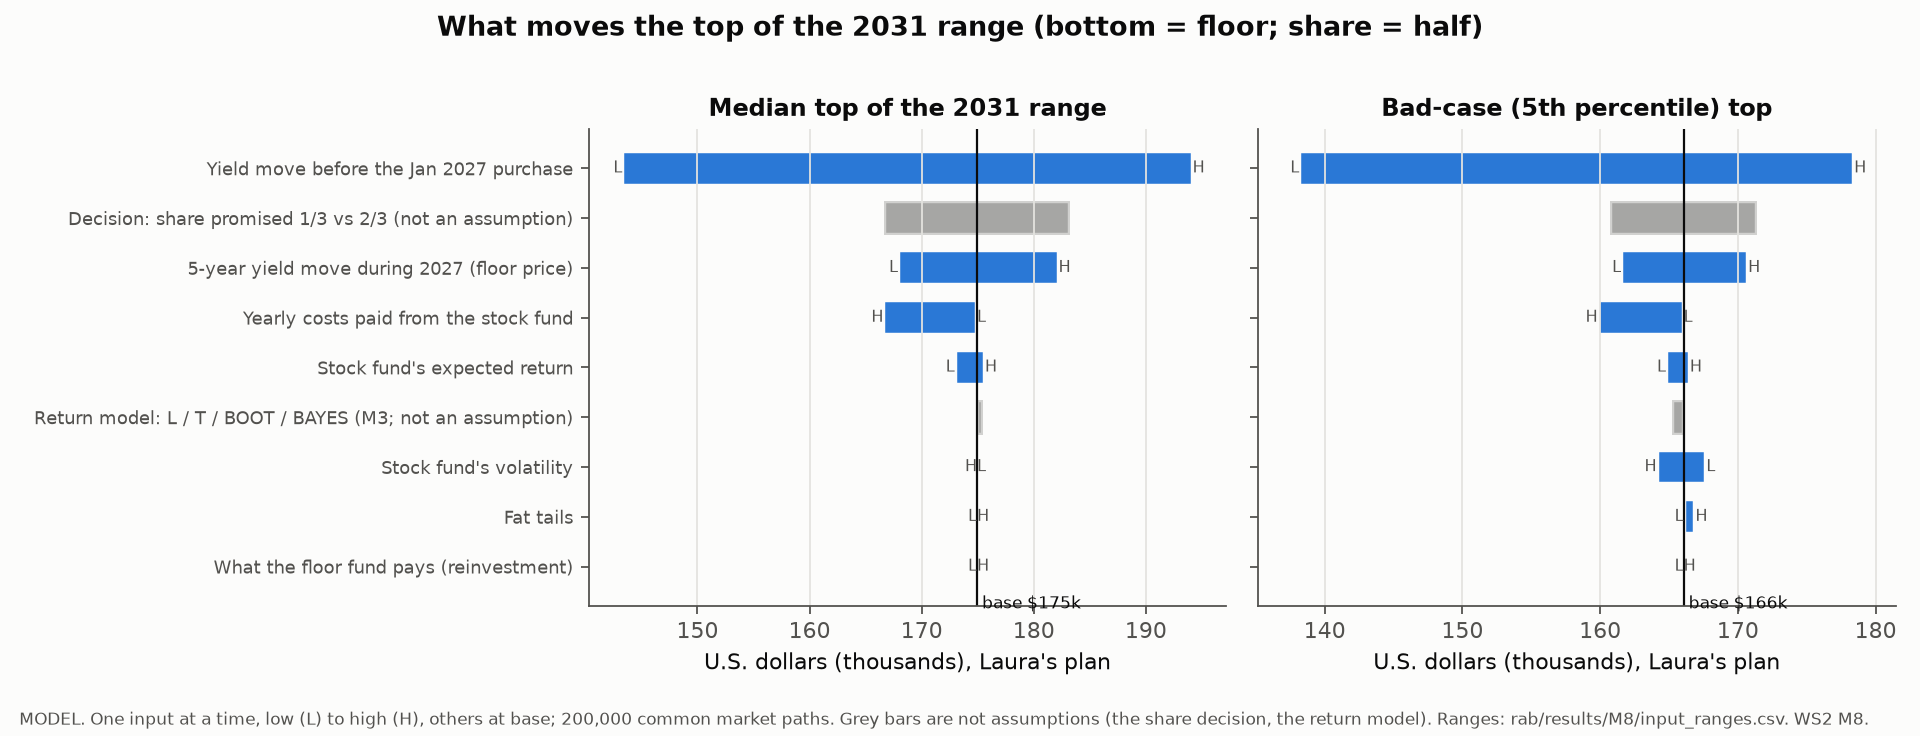
\includegraphics[width=\textwidth]{M8/fig_M8_tornado.png}
\caption{Tornado for the top of the 2031 range (M8, MODEL). Grey bars are not assumptions: the share decision and
the choice of return model.}
\label{fig:tornado}
\end{figure}

The lesson for the IPS is simple: the range depends on interest rates on two dates, and on fees, far more than on how
stocks do. So the IPS should name those two rate dates and the rule that costs come from the stock fund, not the
floor; the stock-return forecast barely matters.

% =====================================================================================================
\FloatBarrier
\section{Decisions}\label{sec:decisions}

Nothing in this paper changes the strategy. Table~\ref{tab:decisions} collects the decisions the team must ratify,
with the kit's recommendation and the classification required by the contradiction rule. Memos are in
\texttt{rab/decisions/}; the IPS edit ledger (\texttt{D\_ips\_edit\_ledger.md}) holds the word budget.

\begin{table}[h]
\centering\small
\begin{tabularx}{\textwidth}{>{\raggedright}p{2.8cm}>{\raggedright}X>{\raggedright}p{1.75cm}>{\raggedright\arraybackslash}p{3.0cm}}
\toprule
Decision (memo) & Kit recommendation & Confidence & Class; decide by \\
\midrule
WInS book (D7) & The \texttt{Portfolio} tab: shows all three of Laura's goals before the 23 Oct Trading Notes & -- & team vote, 1 Oct \\
Pre-2027 hedge & Do not hedge; buy at once, latest first; 2028 deposit completes any gap & High & note in Final Report \\
Share promised (D6) & Keep half & High (STRIPS), medium (Book L) & none for the share; 26 Oct \\
Who covers a coupon shortfall & Name one owner inside the portfolio (kit: Laura's half first, then the gift above the floor, then the floor); never ``her own money'' & Medium & fix before 6 Nov (IPS cushion sentence); 26 Oct \\
Certainty definition & Structure plus a named cover: Treasuries maturing \emph{before} each payment, held to maturity; the government owes most of each payment; a named part covers a reinvestment shortfall & High & fix before 6 Nov (replace ``just before'' sentence); 20 Oct \\
Coupon policy & Replace ``needs no rebalancing'': each holding's income buys Treasuries for the same payment & High & fix before 6 Nov \\
2031 range confidence & ``Inside the range by construction, if'' five conditions; floor quoted rounded down (\$145,000 today) & High & fix before 6 Nov (``rounded down'') \\
Assumptions to state & Jan 2027 yields (already covered), Jan 2028 5-year yield (optional), costs paid by the stock fund & High & fix before 6 Nov (costs only) \\
Floor definition (F4) & Which pocket absorbs a pre-2028 yield fall: floor or stock fund & -- & fix before 6 Nov; 14 Oct \\
Stock fund & Keep VT & High that it barely matters & note in Final Report \\
Rivals & Keep Root-and-Branch; name All-Treasury as closest & High & note in Final Report \\
Bad-year clause & Sell nothing; a stock fall triggers no trade & High & fix before 6 Nov (wording, with the coupon policy) \\
Literature challenges & Stocks are not safe over long horizons \citep{anarkulova2022stocks,bodie1995risk}; TIPS--Treasury mispricing \citep{fleckenstein2014tips} & -- & note in Final Report; ignore (not available) \\
\bottomrule
\end{tabularx}
\caption{Decisions to ratify. ``Fix before 6 Nov'' items are wording only; the IPS has about 17 spare words against
about 21--36 needed, so the ledger pairs them with candidate cuts.}
\label{tab:decisions}
\end{table}
\keys{\nk{ws3.ips.word_count_30sep}, \src{rab/decisions/D_ips_edit_ledger.md}, \nk{ws2.range.announced_floor}, \nk{ws2.range.floor_reading}}

\textbf{What the team can say.} ``High certainty'' means Treasuries maturing before each payment, bought in January
2027 and held to maturity; the government owes at least about \$42,000 of every \$50,000 and, with coupons reinvested
near today's yields, all of it; a named part of the portfolio covers any shortfall before the facility gift. The 2031
range runs from the floor, quoted rounded down, to the floor plus half the fund; the gift lands inside by construction
and, in the models, near the top about 3 times in 4. Numeric ranges build more trust than vague words
\citep{vanderbles2020trust}, and a picture with a solid floor and a shaded upside helps non-experts
\citep{spiegelhalter2011visualizing}.

% =====================================================================================================
\section{Limitations}\label{sec:limits}

\begin{itemize}
  \item \textbf{One curve, one day, model prices.} Everything is on the 28 September 2026 curve with no dealer mark-up.
  The ladder cost and the odds move with rates; re-run M1, M2 and M8 on Friday's curve before quoting dollars.
  \item \textbf{STRIPS basis for M2--M8.} Only M1 section E and the D6 coupon checks model the coupon ladder. The
  pairing of coupon gaps with stress episodes is by hand and single-build; the 1962--2011 coupon replay is one build
  (\UNV).
  \item \textbf{Independence assumptions.} M3, M4 and M8 treat stocks and yields as unlinked and 2027 and 2028 yields as
  independent; bad stock years and falling yields often coincide.
  \item \textbf{U.S. history stands in for a world fund.} The history lens keeps today's 62\% U.S. weight in every year,
  and the U.S. market was unusually good \citep{anarkulova2022stocks}; M3 re-centres its bootstrap on 7.0\% for that
  reason. Pre-1962 curves are flat at the long rate.
  \item \textbf{Value judgements.} The D6 rule's 10\% cushion and 95\% level, and the fund switch bar, are judgements
  fixed in advance, not facts.
  \item \textbf{Rules not yet seen in WInS.} Bond quantity units, accrued conventions, exact names of IBTO--IBTR and the
  bonds, order types, and whether low-coupon bonds are listed are \UNV{} until the team sees them in WInS.
  \item \textbf{Not modelled.} Yields falling after 2031; an early close or drift of an iBonds fund; a U.S. payment
  delay longer than the 47 days from 15 November to 1 January; currency risk on a gift spent in Taiwan; taxes (outside
  the case).
  \item \textbf{Literature.} Some references were checked only through a secondary source (marked S in
  \texttt{rab/literature/references.md}); the team should read those before quoting them.
\end{itemize}

\FloatBarrier
\label{lastmainpage}
\renewcommand{\bibfont}{\small\raggedright}
\bibliographystyle{plainnat}
\bibliography{../literature/references}

% =====================================================================================================
\clearpage
\appendix
\section{Model cards}\label{app:cards}
% Model cards, condensed from rab/models/M*_CARD.md, M1_METHOD.md and rab/trades/M9_selection.md (30 Sep 2026).
% Full cards and specs live next to the code; these are summaries. All outputs MODEL, 28 Sep 2026 curve, seed 20260930.
\small
\newcommand{\card}[2]{\par\medskip\noindent\colorbox{black!6}{\parbox{\dimexpr\textwidth-2\fboxsep}{\textbf{#1}\hfill{\footnotesize #2}}}\par\smallskip}
\newcommand{\cf}[1]{\textbf{#1.}~}

\card{M1 Ladder pricer}{spec \texttt{M1\_METHOD.md}; code \texttt{m1\_ladder.py}; out \texttt{rab/models/out/}}
\cf{Question} What the ten payments and the WInS book cost on the reference curve; whether WInS bond prices are fair.
\cf{Method} Par curve on a half-year grid (linear), bootstrapped to discount factors, log-linear interpolation;
payments valued on the Nov-15 STRIPS basis (headline) and on the exact dates; forward to 1 Jan 2027 and 2028; book
costed with commissions; bond yield check (flag beyond 25bp); iBonds look-through; coupon reinvestment stress (section E);
cost-of-certainty history on every curve since 1990 (section G).
\cf{Data} Treasury par curve 28 Sep 2026; WInS prices recorded 28--29 Sep; iShares facts; Nasdaq closes.
\cf{Limits} Model prices, no dealer mark-up; one curve, one day; WInS settlement, bond unit and accrued conventions \UNV;
history keeps today's time to maturity. \cf{Failure mode} quoting the exact-date value (not buyable) as the cost.
\cf{Verification} Gate A: four builders, maximum difference \$0.00 on every headline.

\card{M2 Rate paths to January 2027}{spec \texttt{M2\_SPEC.md}; code \texttt{m2\_rate\_paths.py}; out \texttt{results/M2/}}
\cf{Question} The chance the ten payments cost more than \$300,000 on 1 Jan 2027, and whether to hedge.
\cf{Method} Five estimators with no view on direction (rescaled history since 1963; history at similar yield levels;
bias-corrected Vasicek AR(1); three-factor PCA + VAR(1); MOVE-calibrated options volatility); headline = their median.
\cf{Data} Treasury par curves 1990--2026, FRED constant maturity 1962--1989, MOVE (secondary source).
\cf{Limits} A quarter-by-quarter figure that moves with volatility; STRIPS basis only; fitted mean reversion is
indistinguishable from none. \cf{Failure mode} quoting a decimal, or quoting the superseded 24.2\%.
\cf{Verification} Gate B (WS4): blind rebuild within 0.005 points on decision keys; third standard-library pricer agrees.

\card{M3 Branch Monte Carlo}{spec \texttt{M3\_SPEC.md}; code \texttt{m3\_branch.py}; out \texttt{results/M3/}}
\cf{Question} The 2031 range top and the 2033 gift under the adopted rule.
\cf{Method} 200,000 paths per model: Student-$t$ ($\nu=4$), Shiller block bootstrap (24-month blocks, re-centred on
7.0\%), Bayesian uncertain mean (PyMC, $\hat r\le1.001$), lognormal reference reproducing insight\_v1.
\cf{Data} Shiller monthly 1871--2026; Damodaran 1928--2025; J.P.~Morgan 2026 LTCMA (world stocks 7.00\%).
\cf{Limits} U.S. history stands in for VT; no link between stocks and rates; floor taken at face (M4 relaxes this).
\cf{Failure mode} reading the model percentile as the confidence that the gift lands in the range (that is by construction).
\cf{Verification} Gate B (WS2): median top within \$34, probability of reaching the top within 0.12 points.

\card{M4 Cap optimiser (D6)}{spec \texttt{M4\_SPEC.md} s5 (rule committed first, 3d98ce0); code \texttt{m4\_cap.py}}
\cf{Question} What share of the stock fund to promise at the top of the 2031 range.
\cf{Method} Pre-registered rule: largest share with the gift above the announced floor in 99.5\% of paths and Laura
keeping $\ge$10\% of her gift in 95\%, in all three decision models; keep half if the answer is in 0.40--0.60. Floor
delivery modelled with historical reinvestment rates and the fund fee; announced floor = worst case rounded down to
\$5,000. NSGA-II (pymoo) front as an indicative check. Coupon-gap variants with three owners (\texttt{m4\_gap\_owner.py}).
\cf{Limits} The 10\% and 95\% are value judgements; 0 in 200,000 is not proof of impossibility.
\cf{Verification} Gate B (WS2): same answer (0.50 / 0.47 / 0.47) in both builds and on ten more seeds.

\card{M5 Century backtest}{spec \texttt{M5\_SPEC.md}; code \texttt{m5\_backtest.py}; out \texttt{results/M5/}}
\cf{Question} The price of certainty on every curve since 1871, and the plan replayed from 149 start years.
\cf{Method} M1's pricer on daily (1962+) and month-start (1871+) curves; each start year's yields buy the ladder and
floor and its returns drive the fund; second view with today's yields and history's returns.
\cf{Data} Treasury and FRED curves; Shiller long rate (flat curve before 1962); Damodaran, JST, French returns; CPI.
\cf{Limits} Flat pre-1962 curves overstate cost by a median 0.8\%; a fixed 62\% U.S. weight; annual steps; no fees.
\cf{Failure mode} reading the history-yield gift (median about \$132,000) as today's outlook.
\cf{Verification} Gate B (WS3): blind rebuild identical to the cent on 19,685 rows.

\card{M6 Rivals and fund choice}{spec \texttt{M6\_SPEC.md} (switch rule first); code \texttt{m6\_rivals.py}}
\cf{Question} Does any rival plan, or any alternative to VT, do better on the case's own tests?
\cf{Method} Same money and payments for eight rivals (all-Treasury, 60/40, ladder + 60/40, glide paths, CPPI $m=3,5$,
TIPS ladder); history lens (149 start years) and J.P.~Morgan Monte Carlo (200,000 paths); four fund alternatives
against a pre-registered switch rule.
\cf{Limits} Lognormal MC without fat tails; gold fixed before 1971 and home prices as a REIT proxy in history.
\cf{Failure mode} comparing gifts instead of the case's two hard tests; treating a threshold result as a decision.
\cf{Verification} Gate B (WS3): history to the cent; MC within 0.85\%; gold/REIT on the line in both builds.

\card{M7 Stress}{spec \texttt{M7\_SPEC.md}; code \texttt{m7\_stress.py}; out \texttt{results/M7/}}
\cf{Question} What bad episodes do to the payments, the floor and the gift; the real value of the payments.
\cf{Method} Today's curve shifted as in each episode; episode stock returns through the fund; adopted rules
applied; thresholds solved for a parallel fall; inflation paths from market breakevens, forecasts and history.
\cf{Limits} Parallel shifts only; foreign episodes in local currency; zero-coupon rungs; payment delays not modelled.
\cf{Failure mode} reading the Great Depression's high real gift as good news (deflation).
\cf{Verification} Gate B (WS3): every scenario, threshold and real value reproduced to the cent.

\card{M8 Sensitivity}{spec \texttt{M8\_SPEC.md}; code \texttt{m8\_sensitivity.py}; out \texttt{results/M8/}}
\cf{Question} Which assumptions move the 2031 range, and which three the IPS must state.
\cf{Method} Full chain from the Jan 2027 purchase to the 2031 range with M1's pricer; tornado on 200,000 common paths;
Sobol total-order indices (SALib); pre-registered selection rule.
\cf{Limits} Inputs independent; uniform ranges for return, volatility and fee are judgements.
\cf{Verification} Gate B (WS2): same three assumptions, same ranking.

\card{M9 Security selection}{\texttt{rab/trades/M9\_selection.md}; code \texttt{m9\_screen.py}}
\cf{Question} Which WInS security best fills each slot, with a runner-up.
\cf{Method} Screen on maturity before the payment, WInS price vs curve (25bp flag), share of cash arriving as coupons
and delivery if coupons earn 0\% or 2\%, cost, the 2$\times$-daily-volume rule, and the exact WInS name (IBTN in WInS is
INSCORP Inc, not an iBond).
\cf{Result} Every \texttt{Portfolio} holding is the best seen in WInS; no order needs splitting; low-coupon 2040 and
2041 bonds are an upgrade if listed.
\cf{Verification} Gate C: 490 checks, 0 failures; reproduces \texttt{reinvest.rung.*} exactly.
\normalsize


\clearpage
\section{Gate tables}\label{app:gates}
% Gate tables, condensed from rab/gates/gate_A.md, gate_B_ws2/ws3/ws4.md, gate_C.md, gate_D.md (30 Sep 2026).
\small
Gates follow \texttt{RUN\_PLAN.md} s3: A (data), B (models), C (trade kit), D (red team). Each is go / fix / stop.

\subsection*{Gate A (data): PASS}
\begin{center}
\begin{tabular}{lcccc}
\toprule
Quantity (28 Sep 2026 curve, MODEL) & Primary & Blind 1 & Blind 2 & Third \\
\midrule
Ten payments, Nov-15 STRIPS basis (headline) & \$289,119.20 & \$289,119.20 & \$289,119.20 & \$289,119.20 \\
Ten payments, exact 1 Jan basis (not buyable) & \$287,016.47 & \$287,016.47 & \$287,016.47 & \$287,016.47 \\
\texttt{Portfolio} book, incl.\ \$200 commission & \$294,764.50 & \$294,764.50 & \$294,764.50 & \$294,764.50 \\
\bottomrule
\end{tabular}
\end{center}
Maximum difference \$0.00. Primary vs blind 1: 65 numbers and 8 dates identical. A first-round \$2,102.73 gap was two
builders reporting different bases; the spec now fixes the headline basis. \texttt{numbers.yaml} locked with a hash
(\texttt{rab/numbers.lock}); the lock re-runs byte for byte.
\keys{\nk{laura.ladder.cost_today_strips}, \nk{laura.ladder.value_today_exact}, \nk{wins.portfolio.cost_close_0928}}

\subsection*{Gate B (models): PASS in all three streams}
\begin{center}
\begin{tabularx}{\textwidth}{>{\raggedright}p{2.5cm}>{\raggedright}p{3.0cm}>{\raggedright\arraybackslash}X}
\toprule
Stream (models) & Rows compared & Result \\
\midrule
WS2 (M3, M4, M8) & 307 blind keys; 29 primary headline keys & 53 match, 247 within tolerance, 7 report-only, 0 outside. Decision numbers identical: $s^*$ 0.50/0.47/0.47, floor \$145,000, the same three IPS assumptions. Rule code gives the other build's numbers exactly on its paths. \\
WS3 (M5, M6, M7) & 278 keys; 19,685 deterministic rows & 204 match, 74 Monte Carlo noise, 0 unreconciled. Deterministic figures to the cent; MC percentiles within 0.85\%, probabilities within 0.16 points. Three reference bugs fixed, none changing a headline. \\
WS4 (M2) & 115 rows & 94 match, 21 within tolerance, 0 unreconciled. Decision keys within 0.005 points and \$0.00; a third standard-library pricer agrees on all 29 comparisons. \\
\bottomrule
\end{tabularx}
\end{center}
Tolerances were fixed in advance: range ends $\pm$2\%, probabilities $\pm$2 points. Records:
\texttt{rab/gates/gate\_B\_ws2.md}, \texttt{gate\_B\_ws3.md}, \texttt{gate\_B\_ws4.md}.

\subsection*{Gate C (trade kit): PASS for the kit}
490 automated checks, 0 failures; 18 \UNV{} (WInS name strings not yet seen), 16 conditional, 31 stale (the live
Sheet tab, to be rewritten before Friday). Checks: note length ($\le$300 characters; longest exemplar 294), exact
ticker names (no IBTN), cash never negative in the order sequence (lowest worst case \$2,445.28 for the
\texttt{Portfolio} book), every order at most 1.2\% of the 2$\times$-volume limit, every number traced to
\texttt{numbers.yaml}; the kit rebuilds byte-identical. Record: \texttt{rab/gates/gate\_C.md}.

\subsection*{Gate D (red team): PASS}
Four red-team reports (three-judge panel, devil's advocate, key-assumptions challenge, fact audit) gave 56 items,
43 after de-duplication: \textbf{17 fixed, 25 deferred with an owner and a deadline, 1 rejected}. Every fix is
wording, sequencing, tooling or evidence; the strategy is unchanged. The most important deferred items:
\begin{itemize}
  \item the coupon-shortfall owner chain must end inside the portfolio, never in ``her own money'' (decide with D6, 26 Oct);
  \item the definition of ``a high degree of certainty'' (now drafted in \texttt{D\_certainty\_definition.md}; by 20 Oct);
  \item the IPS word budget: about 40--50 words of edits against 17 spare (ledger with paired cuts);
  \item D6 ``keep half'' re-run with costs charged to the stock fund (before 26 Oct);
  \item the October trigger that would sell VT after a fall (decide by 14 Oct).
\end{itemize}
Record: \texttt{rab/gates/gate\_D.md}, \texttt{rab/redteam/triage.md}.
\normalsize


\clearpage
\section{Number trace}\label{app:trace}
Generated by \texttt{rab/paper/make\_trace.py} from \texttt{rab/numbers.yaml} (Gate A lock, sha256 in
\texttt{rab/numbers.lock}) and the stream files. For each key cited in the text: the file, the status, and the
\texttt{quote\_as} string the team should use. Values in the YAML files are authoritative.
% generated by make_trace.py - do not edit
\footnotesize
\begin{longtable}{>{\raggedright}p{4.2cm}>{\raggedright}p{2.2cm}>{\raggedright}p{2.4cm}>{\raggedright\arraybackslash}p{5.2cm}}
\toprule Key & File & Status & Quote as \\ \midrule \endhead
\texttt{wins.\allowbreak{}portfolio.\allowbreak{}cost\_\allowbreak{}close\_\allowbreak{}0928} & \texttt{numbers.yaml} & MODEL & about \$294,800 including \$200 commission \\
\texttt{wins.\allowbreak{}portfolio.\allowbreak{}split\_\allowbreak{}close\_\allowbreak{}0928} & \texttt{numbers.yaml} & MODEL & dated Treasury holdings 90\%, world stock fund 9\%, cash 2\% \\
\texttt{wins.\allowbreak{}portfolio.\allowbreak{}holdings\_\allowbreak{}close\_\allowbreak{}0928} & \texttt{numbers.yaml} & MODEL & use percentages in notes (e.g. IBTM about a third of the book) \\
\texttt{market.\allowbreak{}par\_\allowbreak{}curve} & \texttt{numbers.yaml} & VERIFIED-PRIMARY & 10-year Treasury yield 5.24\% on 2026-09-28 \\
\texttt{wins.\allowbreak{}bond\_\allowbreak{}check.\allowbreak{}T\_\allowbreak{}3.\allowbreak{}125\%\_\allowbreak{}15-Nov-2041} & \texttt{numbers.yaml} & MODEL (price SEEN via Sheet) & within 25bp of the curve \\
\texttt{wins.\allowbreak{}bond\_\allowbreak{}check.\allowbreak{}T\_\allowbreak{}4.\allowbreak{}250\%\_\allowbreak{}15-Nov-2040} & \texttt{numbers.yaml} & MODEL (price SEEN via Sheet) & within 25bp of the curve \\
\texttt{wins.\allowbreak{}bond\_\allowbreak{}check.\allowbreak{}T\_\allowbreak{}4.\allowbreak{}375\%\_\allowbreak{}15-Feb-2038} & \texttt{numbers.yaml} & MODEL (price UNVERIFIED, reported stale) & FLAG: price about 1 point of yield off the curve; do not trade at it \\
\texttt{wins.\allowbreak{}bond\_\allowbreak{}check.\allowbreak{}T\_\allowbreak{}4.\allowbreak{}375\%\_\allowbreak{}15-Nov-2039} & \texttt{numbers.yaml} & MODEL (price SEEN via Sheet) & within 25bp of the curve \\
\texttt{wins.\allowbreak{}bond\_\allowbreak{}check.\allowbreak{}T\_\allowbreak{}4.\allowbreak{}500\%\_\allowbreak{}15-Feb-2036} & \texttt{numbers.yaml} & MODEL (price UNVERIFIED, reported stale) & FLAG: price about 1 point of yield off the curve; do not trade at it \\
\texttt{wins.\allowbreak{}bond\_\allowbreak{}check.\allowbreak{}T\_\allowbreak{}4.\allowbreak{}500\%\_\allowbreak{}15-May-2038} & \texttt{numbers.yaml} & MODEL (price SEEN via Sheet) & within 25bp of the curve \\
\texttt{wins.\allowbreak{}bond\_\allowbreak{}check.\allowbreak{}T\_\allowbreak{}4.\allowbreak{}750\%\_\allowbreak{}15-Feb-2037} & \texttt{numbers.yaml} & MODEL (price SEEN via Sheet) & within 25bp of the curve \\
\texttt{market.\allowbreak{}etf\_\allowbreak{}2026-09-28} & \texttt{numbers.yaml} & VERIFIED-PRIMARY (Nasdaq consolidated; WInS close where seen & quote prices only with their date \\
\texttt{ws3.\allowbreak{}inputs.\allowbreak{}mc} & \texttt{numbers\_ws3.yaml} & GATE B (stream file) & J.P. Morgan 2026: world stocks 7.0\% a year; Treasuries at today's 5.06\% five-year yield \\
\texttt{laura.\allowbreak{}ladder.\allowbreak{}cost\_\allowbreak{}today\_\allowbreak{}strips} & \texttt{numbers.yaml} & MODEL & about \$289,000 at 2026-09-28 yields \\
\texttt{laura.\allowbreak{}ladder.\allowbreak{}cost\_\allowbreak{}2027\_\allowbreak{}strips} & \texttt{numbers.yaml} & MODEL & about \$292,000 on 1 Jan 2027, at 28 Sep 2026 yields \\
\texttt{laura.\allowbreak{}ladder.\allowbreak{}headroom\_\allowbreak{}2027\_\allowbreak{}strips} & \texttt{numbers.yaml} & MODEL & about \$7,600 of room under \$300,000 \\
\texttt{laura.\allowbreak{}ladder.\allowbreak{}breakeven\_\allowbreak{}fall\_\allowbreak{}bp\_\allowbreak{}strips} & \texttt{numbers.yaml} & MODEL & yields would have to fall about a quarter of a percentage point (about 26bp) before 1 Jan 2027 \\
\texttt{laura.\allowbreak{}ladder.\allowbreak{}value\_\allowbreak{}today\_\allowbreak{}exact} & \texttt{numbers.yaml} & MODEL & about \$287,000 \\
\texttt{laura.\allowbreak{}ladder.\allowbreak{}value\_\allowbreak{}2027\_\allowbreak{}exact} & \texttt{numbers.yaml} & MODEL & about \$290,000 on 1 Jan 2027 \\
\texttt{laura.\allowbreak{}ladder.\allowbreak{}cost\_\allowbreak{}2027\_\allowbreak{}strips\_\allowbreak{}model\_\allowbreak{}band} & \texttt{numbers.yaml} & MODEL & \$292,000 give or take \$300 across reasonable curve methods \\
\texttt{laura.\allowbreak{}ladder.\allowbreak{}gpt\_\allowbreak{}check} & \texttt{numbers.yaml} & REPRODUCED & an independent check agreed within about \$200 \\
\texttt{laura.\allowbreak{}plan\_\allowbreak{}split\_\allowbreak{}2028.\allowbreak{}strips} & \texttt{numbers.yaml} & MODEL & ladder 66\%, floor 25\%, stock fund 9\% \\
\texttt{laura.\allowbreak{}floor\_\allowbreak{}cost\_\allowbreak{}2028} & \texttt{numbers.yaml} & MODEL & about \$117,000 buys the \$150,000 floor (at 28 Sep 5-year yield) \\
\texttt{laura.\allowbreak{}stock\_\allowbreak{}fund\_\allowbreak{}2028\_\allowbreak{}usd.\allowbreak{}strips} & \texttt{numbers.yaml} & MODEL & about \$41,000 \\
\texttt{wins.\allowbreak{}portfolio.\allowbreak{}targets\_\allowbreak{}typed} & \texttt{numbers.yaml} & SEEN (Sheet, 30 Sep) & the ladder is about two-thirds of the WInS book \\
\texttt{history.\allowbreak{}days\_\allowbreak{}priced\_\allowbreak{}since\_\allowbreak{}2000} & \texttt{numbers.yaml} & REPRODUCED & every daily Treasury curve since 2000 (about 6,700 days) \\
\texttt{history.\allowbreak{}share\_\allowbreak{}days\_\allowbreak{}le\_\allowbreak{}300k} & \texttt{numbers.yaml} & REPRODUCED & on about 1 day in 9 since 2000 would \$300,000 have bought all ten payments \\
\texttt{history.\allowbreak{}cheapest\_\allowbreak{}since} & \texttt{numbers.yaml} & REPRODUCED & the cheapest since mid-2002 \\
\texttt{history.\allowbreak{}cost\_\allowbreak{}2020\_\allowbreak{}median} & \texttt{numbers.yaml} & REPRODUCED & about \$460,000 at 2020 yields \\
\texttt{history.\allowbreak{}cost\_\allowbreak{}2020\_\allowbreak{}range} & \texttt{numbers.yaml} & REPRODUCED & \$408,000 to \$470,000 during 2020 \\
\texttt{history.\allowbreak{}cost\_\allowbreak{}max} & \texttt{numbers.yaml} & REPRODUCED & about \$470,000 on 4 Aug 2020, the most expensive day since 1990 \\
\texttt{history.\allowbreak{}unfunded\_\allowbreak{}days} & \texttt{numbers.yaml} & REPRODUCED & only at 2020-21 yields would part of one payment have been left unfunded (worst about \$21,000) \\
\texttt{reinvest.\allowbreak{}bookL\_\allowbreak{}delivered} & \texttt{numbers.yaml} & MODEL & coupons reinvested at today's yields: about \$503,000; at 2\%: about \$466,000; at 0\%: about \$447,000 \\
\texttt{reinvest.\allowbreak{}rung.\allowbreak{}IBTM} & \texttt{numbers.yaml} & MODEL & per-rung detail; quote only in the Final Report appendix \\
\texttt{reinvest.\allowbreak{}rung.\allowbreak{}IBTO} & \texttt{numbers.yaml} & MODEL & per-rung detail; quote only in the Final Report appendix \\
\texttt{reinvest.\allowbreak{}rung.\allowbreak{}IBTP} & \texttt{numbers.yaml} & MODEL & per-rung detail; quote only in the Final Report appendix \\
\texttt{reinvest.\allowbreak{}rung.\allowbreak{}IBTQ} & \texttt{numbers.yaml} & MODEL & per-rung detail; quote only in the Final Report appendix \\
\texttt{reinvest.\allowbreak{}rung.\allowbreak{}IBTR} & \texttt{numbers.yaml} & MODEL & per-rung detail; quote only in the Final Report appendix \\
\texttt{reinvest.\allowbreak{}rung.\allowbreak{}T\_\allowbreak{}3.\allowbreak{}125\%\_\allowbreak{}15-Nov-2041} & \texttt{numbers.yaml} & MODEL & per-rung detail; quote only in the Final Report appendix \\
\texttt{reinvest.\allowbreak{}rung.\allowbreak{}T\_\allowbreak{}4.\allowbreak{}250\%\_\allowbreak{}15-Nov-2040} & \texttt{numbers.yaml} & MODEL & per-rung detail; quote only in the Final Report appendix \\
\texttt{reinvest.\allowbreak{}rung.\allowbreak{}T\_\allowbreak{}4.\allowbreak{}375\%\_\allowbreak{}15-Nov-2039} & \texttt{numbers.yaml} & MODEL & per-rung detail; quote only in the Final Report appendix \\
\texttt{reinvest.\allowbreak{}rung.\allowbreak{}T\_\allowbreak{}4.\allowbreak{}500\%\_\allowbreak{}15-May-2038} & \texttt{numbers.yaml} & MODEL & per-rung detail; quote only in the Final Report appendix \\
\texttt{reinvest.\allowbreak{}rung.\allowbreak{}T\_\allowbreak{}4.\allowbreak{}750\%\_\allowbreak{}15-Feb-2037} & \texttt{numbers.yaml} & MODEL & per-rung detail; quote only in the Final Report appendix \\
\texttt{reinvest.\allowbreak{}bookL\_\allowbreak{}buffer\_\allowbreak{}cost} & \texttt{numbers.yaml} & MODEL & about \$20,000 more today keeps every payment whole if coupons earn only 2\% \\
\texttt{ws3.\allowbreak{}external.\allowbreak{}ws7\_\allowbreak{}coupon\_\allowbreak{}reinvestment} & \texttt{numbers\_ws3.yaml} & GATE B (stream file) & the WInS book's ten payments total \$500,000 only if coupons are reinvested at about 5\% (4.97\%) or more \\
\texttt{ws4.\allowbreak{}bookL\_\allowbreak{}cost\_\allowbreak{}resized} & \texttt{numbers\_ws4.yaml} & DERIVED (MODEL) from the Gate-A-passed M1 output; stdlib and & sized to pay exactly \$50,000 a year, the WInS-listed ladder costs about \$289,200, within \$100 of STRIPS \\
\texttt{ws2.\allowbreak{}range.\allowbreak{}top2031} & \texttt{numbers\_ws2.yaml} & GATE B (stream file) & a top of about \$175,000 in a typical case; 90\% of paths about \$165,000-\$190,000 (MODEL, at 28 Sep 2026 yields) \\
\texttt{ws2.\allowbreak{}range.\allowbreak{}gift\_\allowbreak{}inside\_\allowbreak{}range} & \texttt{numbers\_ws2.yaml} & GATE B (stream file) & certain by construction if the floor holding pays, the 2028 deposit arrives, the gift is capped and no fee is taken from the floor; no model path fell outside \\
\texttt{ws2.\allowbreak{}range.\allowbreak{}p\_\allowbreak{}fund\_\allowbreak{}holds\_\allowbreak{}2031\_\allowbreak{}to\_\allowbreak{}2033} & \texttt{numbers\_ws2.yaml} & GATE B (stream file) & about 3 times in 4 the stock fund is worth at least its 2031 value in 2033, and the gift then lands at the top or within about \$3,700 of it (MODEL) \\
\texttt{ws2.\allowbreak{}range.\allowbreak{}expected\_\allowbreak{}short\_\allowbreak{}of\_\allowbreak{}top} & \texttt{numbers\_ws2.yaml} & GATE B (stream file) & on average the gift ends about \$2,000 below the top (MODEL) \\
\texttt{ws2.\allowbreak{}range.\allowbreak{}p\_\allowbreak{}below\_\allowbreak{}middle} & \texttt{numbers\_ws2.yaml} & GATE B (stream file) & below the middle of the range at most about 1 time in 200 (MODEL, history model) \\
\texttt{ws2.\allowbreak{}range.\allowbreak{}p\_\allowbreak{}fund\_\allowbreak{}below\_\allowbreak{}cost\_\allowbreak{}2031} & \texttt{numbers\_ws2.yaml} & GATE B (stream file) & in about 1 case in 5 the fund is worth less in 2031 than it cost in 2028; the range is then narrower but its bottom does not move (MODEL) \\
\texttt{ws2.\allowbreak{}range.\allowbreak{}floor\_\allowbreak{}delivery} & \texttt{numbers\_ws2.yaml} & GATE B (stream file) & the floor pays about \$149,000 in a typical case and at least about \$146,000; it falls short of \$150,000 about 2 times in 3 (MODEL) \\
\texttt{ws2.\allowbreak{}range.\allowbreak{}announced\_\allowbreak{}floor} & \texttt{numbers\_ws2.yaml} & GATE B (stream file) & \$145,000: the floor holding's worst case, rounded down to \$5,000 \\
\texttt{ws2.\allowbreak{}range.\allowbreak{}floor\_\allowbreak{}shortfall\_\allowbreak{}vs\_\allowbreak{}face} & \texttt{numbers\_ws2.yaml} & DERIVED & typically about \$600, at most about \$3,700 (MODEL) \\
\texttt{ws2.\allowbreak{}d6.\allowbreak{}s\_\allowbreak{}star} & \texttt{numbers\_ws2.yaml} & GATE B (stream file) & the largest share that passes both tests is 0.47-0.50 (MODEL) \\
\texttt{ws2.\allowbreak{}d6.\allowbreak{}decision\_\allowbreak{}share} & \texttt{numbers\_ws2.yaml} & GATE B (stream file) & keep half (D6, to ratify at the 26 Oct meeting) \\
\texttt{ws2.\allowbreak{}d6.\allowbreak{}p\_\allowbreak{}gift\_\allowbreak{}below\_\allowbreak{}145k\_\allowbreak{}any\_\allowbreak{}share} & \texttt{numbers\_ws2.yaml} & GATE B (stream file) & no model path puts the gift below \$145,000 at any share (0 in 200,000 per model; not proof) \\
\texttt{ws2.\allowbreak{}d6.\allowbreak{}options} & \texttt{numbers\_ws2.yaml} & GATE B (stream file) & see the D6 memo table (round to \$1k; probabilities to whole percent) \\
\texttt{ws2.\allowbreak{}d6.\allowbreak{}rule\_\allowbreak{}sensitivity} & \texttt{numbers\_ws2.yaml} & GATE B (stream file) & a 5\% cushion would allow about 2/3; a 15\% cushion about 1/5 (MODEL) \\
\texttt{ws2.\allowbreak{}d6.\allowbreak{}half\_\allowbreak{}vs\_\allowbreak{}047\_\allowbreak{}expected\_\allowbreak{}gift} & \texttt{numbers\_ws2.yaml} & DERIVED & about \$1,500 more expected gift at half than at 0.47 (MODEL) \\
\texttt{ws2.\allowbreak{}d6.\allowbreak{}gap\_\allowbreak{}owner} & \texttt{numbers\_ws2.yaml} & GATE B (stream file) & with Laura's half paying a coupon shortfall first (WS3 rule 3), the rule keeps half at today's yields (largest passing share 0.42 in all three models) and the 2031 top is never lowered; at yields 2 points lower no share passes under any owner, the top is lowered in 7-10\% of paths, and the gift falls below \$145,000 in at most about 1 path in 300 (MODEL) \\
\texttt{ws2.\allowbreak{}d6.\allowbreak{}gap\_\allowbreak{}owner\_\allowbreak{}tolerance} & \texttt{numbers\_ws2.yaml} & GATE B (stream file) & with Laura's half paying first, the rule keeps half for a 2031 gap up to about \$2,200 (about \$4,700 if the whole fund paid first); no share passes above about \$14,500 (MODEL) \\
\texttt{ws2.\allowbreak{}d6.\allowbreak{}ladder\_\allowbreak{}gap} & \texttt{numbers\_ws2.yaml} & GATE B (stream file) & if Laura's real ladder is the WInS-listed Book L and its coupons are reinvested at today's yields, the gap is about \$1,600 and the rule still keeps half; at yields 2 points lower the gap is about \$18,000 and no share passes, not even zero; the gift falls below \$145,000 (payments first) at most about 1 time in 300 at that level, 1-3\% of paths if coupons earn 2\%, about 1 in 3 at 0\% (MODEL) \\
\texttt{ws3.\allowbreak{}rivals.\allowbreak{}REC} & \texttt{numbers\_ws3.yaml} & GATE B (stream file) & Root-and-Branch (adopted): quote only as a row of the Final Report rivals table \\
\texttt{ws3.\allowbreak{}rivals.\allowbreak{}R1} & \texttt{numbers\_ws3.yaml} & GATE B (stream file) & All-Treasury: quote only as a row of the Final Report rivals table \\
\texttt{ws3.\allowbreak{}rivals.\allowbreak{}R2} & \texttt{numbers\_ws3.yaml} & GATE B (stream file) & 60/40 whole portfolio: quote only as a row of the Final Report rivals table \\
\texttt{ws3.\allowbreak{}rivals.\allowbreak{}R3} & \texttt{numbers\_ws3.yaml} & GATE B (stream file) & Ladder + 60/40 growth money: quote only as a row of the Final Report rivals table \\
\texttt{ws3.\allowbreak{}rivals.\allowbreak{}R4} & \texttt{numbers\_ws3.yaml} & GATE B (stream file) & Glide path 65->20: quote only as a row of the Final Report rivals table \\
\texttt{ws3.\allowbreak{}rivals.\allowbreak{}R4b} & \texttt{numbers\_ws3.yaml} & GATE B (stream file) & Growth-first 75->40: quote only as a row of the Final Report rivals table \\
\texttt{ws3.\allowbreak{}rivals.\allowbreak{}R5} & \texttt{numbers\_ws3.yaml} & GATE B (stream file) & CPPI multiplier 3: quote only as a row of the Final Report rivals table \\
\texttt{ws3.\allowbreak{}rivals.\allowbreak{}R6\_\allowbreak{}tips} & \texttt{numbers\_ws3.yaml} & GATE B (stream file) & a TIPS ladder leaves at least one \$50,000 payment short in most inflation paths \\
\texttt{ws3.\allowbreak{}rivals.\allowbreak{}rec\_\allowbreak{}minus\_\allowbreak{}all\_\allowbreak{}treasury\_\allowbreak{}mc} & \texttt{numbers\_ws3.yaml} & GATE B (stream file) & against all Treasuries, Root-and-Branch gives up about \$9,500 in a bad case for about \$38,000 in a good case \\
\texttt{ws3.\allowbreak{}rivals.\allowbreak{}facility\_\allowbreak{}gift\_\allowbreak{}rec\_\allowbreak{}vs\_\allowbreak{}all\_\allowbreak{}treasury\_\allowbreak{}mc} & \texttt{numbers\_ws3.yaml} & GATE B (stream file) & for the facility alone, All-Treasury gives more at every percentile (about \$28,000 more at the median) \\
\texttt{ws3.\allowbreak{}rivals.\allowbreak{}stress\_\allowbreak{}rec\_\allowbreak{}vs\_\allowbreak{}all\_\allowbreak{}treasury} & \texttt{numbers\_ws3.yaml} & GATE B (stream file) & in a 1929-style crash all Treasuries would end about \$28,000 ahead \\
\texttt{ws3.\allowbreak{}stress.\allowbreak{}S0} & \texttt{numbers\_ws3.yaml} & GATE B (stream file) & quote only in the Final Report stress table \\
\texttt{ws3.\allowbreak{}fund.\allowbreak{}alt.\allowbreak{}A1} & \texttt{numbers\_ws3.yaml} & GATE B (stream file) & VTI + VXUS 62/38: quote only as a row of the Final Report table \\
\texttt{ws3.\allowbreak{}fund.\allowbreak{}alt.\allowbreak{}A2} & \texttt{numbers\_ws3.yaml} & GATE B (stream file) & U.S. only: quote only as a row of the Final Report table \\
\texttt{ws3.\allowbreak{}fund.\allowbreak{}alt.\allowbreak{}A3} & \texttt{numbers\_ws3.yaml} & GATE B (stream file) & VT + small/value tilt: quote only as a row of the Final Report table \\
\texttt{ws3.\allowbreak{}fund.\allowbreak{}alt.\allowbreak{}A4} & \texttt{numbers\_ws3.yaml} & GATE B (stream file) & VT + gold/REIT: quote only as a row of the Final Report table \\
\texttt{ws3.\allowbreak{}fund.\allowbreak{}vt\_\allowbreak{}gift\_\allowbreak{}mc} & \texttt{numbers\_ws3.yaml} & GATE B (stream file) & with VT the bad-case (1 in 20) gift is about \$165,000 and the typical gift about \$174,000 \\
\texttt{ws3.\allowbreak{}fund.\allowbreak{}gold\_\allowbreak{}reit\_\allowbreak{}noise\_\allowbreak{}free} & \texttt{numbers\_ws3.yaml} & GATE B (stream file) & gold/REIT is 0.001 under the 0.90 bar: a close call \\
\texttt{ws3.\allowbreak{}fund.\allowbreak{}gold\_\allowbreak{}reit\_\allowbreak{}etf\_\allowbreak{}lens} & \texttt{numbers\_ws3.yaml} & GATE B (stream file) & on real ETF prices gold/REIT added nothing \\
\texttt{ws3.\allowbreak{}fund.\allowbreak{}max\_\allowbreak{}abs\_\allowbreak{}badcase\_\allowbreak{}change} & \texttt{numbers\_ws3.yaml} & GATE B (stream file) & no alternative moves the bad-case gift by more than about \$1,500 \\
\texttt{ws3.\allowbreak{}stress.\allowbreak{}today\_\allowbreak{}yields\_\allowbreak{}backtest} & \texttt{numbers\_ws3.yaml} & GATE B (stream file) & with today's yields, the worst stretch since 1872 still gives a gift of about \$159,000 \\
\texttt{ws3.\allowbreak{}stress.\allowbreak{}worst\_\allowbreak{}gift\_\allowbreak{}once\_\allowbreak{}floor\_\allowbreak{}bought} & \texttt{numbers\_ws3.yaml} & GATE B (stream file) & once the \$150,000 floor is bought, the worst replay (Great Depression) still gives about \$159,000 \\
\texttt{ws3.\allowbreak{}stress.\allowbreak{}thresholds\_\allowbreak{}bp} & \texttt{numbers\_ws3.yaml} & GATE B (stream file) & the \$150,000 bottom survives a fall in yields of about 1 point before the money arrives; a payment needs a fall of over 4 points \\
\texttt{ws3.\allowbreak{}stress.\allowbreak{}S2b} & \texttt{numbers\_ws3.yaml} & GATE B (stream file) & quote only in the Final Report stress table \\
\texttt{ws3.\allowbreak{}stress.\allowbreak{}S4a} & \texttt{numbers\_ws3.yaml} & GATE B (stream file) & quote only in the Final Report stress table \\
\texttt{ws3.\allowbreak{}stress.\allowbreak{}downgrades\_\allowbreak{}dy10\_\allowbreak{}bp} & \texttt{numbers\_ws3.yaml} & GATE B (stream file) & after the 2011 downgrade the 10-year yield fell about half a point \\
\texttt{ws3.\allowbreak{}stress.\allowbreak{}worst\_\allowbreak{}gift\_\allowbreak{}13\_\allowbreak{}scenarios} & \texttt{numbers\_ws3.yaml} & GATE B (stream file) & the lowest gift in all 13 stress scenarios is about \$147,000 (Japan, with a 1-point fall before Jan 2027) \\
\texttt{ws3.\allowbreak{}stress.\allowbreak{}S6} & \texttt{numbers\_ws3.yaml} & GATE B (stream file) & quote only in the Final Report stress table \\
\texttt{ws3.\allowbreak{}stress.\allowbreak{}S2} & \texttt{numbers\_ws3.yaml} & GATE B (stream file) & quote only in the Final Report stress table \\
\texttt{ws3.\allowbreak{}stress.\allowbreak{}S5} & \texttt{numbers\_ws3.yaml} & GATE B (stream file) & quote only in the Final Report stress table \\
\texttt{ws3.\allowbreak{}stress.\allowbreak{}coupon\_\allowbreak{}gap\_\allowbreak{}vs\_\allowbreak{}laura\_\allowbreak{}half} & \texttt{numbers\_ws3.yaml} & GATE B (stream file) & if coupons earn only 2\% for years, the gap (about \$30,000 in 2033 money) uses up about all of Laura's half in the base case and is about \$12,000-19,000 more than her half after a 2008, 1929 or Japan-style fall \\
\texttt{ws3.\allowbreak{}stress.\allowbreak{}real\_\allowbreak{}value\_\allowbreak{}payments} & \texttt{numbers\_ws3.yaml} & GATE B (stream file) & at the market's expected inflation the last \$50,000 payment buys about what \$35,000 buys in 2027; in a 1970s-style decade about \$18,000 \\
\texttt{ws4.\allowbreak{}gap\_\allowbreak{}odds\_\allowbreak{}2027} & \texttt{numbers\_ws4.yaml} & GATE B (stream file) & about 1 in 3 (MODEL, 28 Sep 2026 curve) \\
\texttt{ws4.\allowbreak{}gap\_\allowbreak{}odds\_\allowbreak{}2027\_\allowbreak{}range} & \texttt{numbers\_ws4.yaml} & GATE B (stream file) & roughly 25-35\% depending on the method \\
\texttt{ws4.\allowbreak{}gap\_\allowbreak{}if\_\allowbreak{}any\_\allowbreak{}typical} & \texttt{numbers\_ws4.yaml} & GATE B (stream file) & if there is a shortfall it is typically about \$10,000 \\
\texttt{ws4.\allowbreak{}gap\_\allowbreak{}p95} & \texttt{numbers\_ws4.yaml} & GATE B (stream file) & in about 1 path in 20 the shortfall is about \$18,000 or more \\
\texttt{ws4.\allowbreak{}p\_\allowbreak{}whole\_\allowbreak{}payment\_\allowbreak{}waits} & \texttt{numbers\_ws4.yaml} & GATE B (stream file) & under 0.3\% \\
\texttt{ws4.\allowbreak{}move\_\allowbreak{}index} & \texttt{numbers\_ws4.yaml} & GATE B (stream file) & not for deliverables (input only) \\
\texttt{ws4.\allowbreak{}stock\_\allowbreak{}fund\_\allowbreak{}2028\_\allowbreak{}median} & \texttt{numbers\_ws4.yaml} & GATE B (stream file) & typically about \$41,000 \\
\texttt{ws4.\allowbreak{}p\_\allowbreak{}stock\_\allowbreak{}fund\_\allowbreak{}below\_\allowbreak{}20k\_\allowbreak{}2028} & \texttt{numbers\_ws4.yaml} & GATE B (stream file) & under \$20,000 in about 1 path in 6 \\
\texttt{ws4.\allowbreak{}perfect\_\allowbreak{}hedge\_\allowbreak{}expected\_\allowbreak{}gain} & \texttt{numbers\_ws4.yaml} & GATE B (stream file) & about \$1,000 at most \\
\texttt{ws4.\allowbreak{}topup\_\allowbreak{}2028\_\allowbreak{}after\_\allowbreak{}150bp\_\allowbreak{}fall} & \texttt{numbers\_ws4.yaml} & GATE B (stream file) & even a 1.5-point fall before January needs only about \$40,000 of the 2028 deposit \\
\texttt{ws2.\allowbreak{}assume.\allowbreak{}sobol\_\allowbreak{}total\_\allowbreak{}index\_\allowbreak{}median\_\allowbreak{}top} & \texttt{numbers\_ws2.yaml} & GATE B (stream file) & yields on 1 Jan 2027 explain about 90\% of the variation in the typical 2031 top; the 5-year yield in Jan 2028 about 7\%; costs about 3\%; the stock-return assumption under 1\% (MODEL) \\
\texttt{ws2.\allowbreak{}assume.\allowbreak{}tornado\_\allowbreak{}median\_\allowbreak{}top} & \texttt{numbers\_ws2.yaml} & GATE B (stream file) & Jan-2027 yields (historical 95-day moves, 2.5-97.5\%) move the typical top from about \$143k to \$194k; the Jan-2028 5-year yield \$168k-\$182k; a 1\% yearly cost \$175k -> \$167k; the stock return (4.1\%-8\%) \$173k-\$176k (MODEL) \\
\texttt{ws2.\allowbreak{}assume.\allowbreak{}luck\_\allowbreak{}share\_\allowbreak{}top2031} & \texttt{numbers\_ws2.yaml} & GATE B (stream file) & stock-market luck explains only about a fifth of the uncertainty in the 2031 top (MODEL) \\
\texttt{ws2.\allowbreak{}assume.\allowbreak{}must\_\allowbreak{}state} & \texttt{numbers\_ws2.yaml} & GATE B (stream file) & (1) yields when the 2027 deposit buys the ten holdings; (2) the 5-year yield when the floor is bought in Jan 2028; (3) costs, and that the stock fund pays them \\
\texttt{ws3.\allowbreak{}ips.\allowbreak{}word\_\allowbreak{}count\_\allowbreak{}30sep} & \texttt{numbers\_ws3.yaml} & GATE B (stream file) & the 30 Sep IPS has about 17 words to spare \\
\texttt{ws2.\allowbreak{}range.\allowbreak{}floor\_\allowbreak{}reading} & \texttt{numbers\_ws2.yaml} & MODEL (deterministic) & after a 0.5-point fall: floor \$143k + fund \$29k under 'the whole remainder', or floor \$150k + fund \$23k under 'keep \$150,000' (MODEL) \\
\bottomrule
\end{longtable}
\normalsize
\noindent Results files cited directly (each reproduced blind at Gate B, or a Gate C record):
\begin{itemize}
\item \texttt{rab/data/MANIFEST.csv}
\item \texttt{rab/results/M5/M5\_report.txt}
\item \texttt{rab/trades/M9\_selection.md}
\item \texttt{rab/results/M2/m2\_estimators.csv}
\item \texttt{rab/decisions/D\_ips\_edit\_ledger.md}
\end{itemize}
\noindent 112 keys, 5 files; 0 missing.


\end{document}
